\documentclass{article}
\usepackage[utf8]{inputenc}
\usepackage{geometry}
\usepackage{enumitem}
\usepackage{hyperref}
\usepackage{xcolor}
\usepackage{graphicx}
\usepackage{array}
\usepackage{multirow}
\usepackage{amsmath, amssymb}
\usepackage{chemfig}
\usepackage{mhchem}
\usepackage{tikz}
\usepackage{setspace}
\usepackage{soul}
\usepackage{mathtools}
\usepackage{booktabs}
\usepackage{chemformula}
\usepackage{siunitx}
\usetikzlibrary{positioning, calc}
\usepackage{longtable}
\geometry{margin=1in}
\setlength{\parskip}{0.5em}
\usepackage{cancel}

\begin{document}

\begin{center}
    {\LARGE\textbf{SI Session Planning Form}}
\end{center}

\vspace{0.5cm}

\noindent
\begin{flushleft}
\textbf{SI Leader:} Brandon Cobb\\
\textbf{Session Week:} 4\\
\textbf{Session\#:} 4\\
\textbf{Instructor:} Professor Tramontozzi\\
\textbf{Old Plans:}\href{https://macombedu.sharepoint.com/:b:/s/ASC-SupplementalInstructionEmbeddedTutoring/EeSYqCwT_KhMolgJvXbVEjgBOyF_DevvS8BgCm1zPkQQJg?e=QJTt4o}{SharePoint}\\
\textbf{Session Goal:} Students will have reviewed unit conversions, algebraic manipulation of exact and inexact numbers, calculating their significant figures after multi-step operations like addition and multiplication. Student will review how to write scienticific notation. Students are given a reference sheet for conversion factors. Students will become adept with atomic particles and subatomic structures like orbitals of electrons. 
\end{flushleft}

\vspace{1em}
\section*{\underline{Opener}}
{\centering\large\textbf{\hl{Take Attendance}}\par}\vspace{-0.25\baselineskip}
\noindent
\begin{tabular}{|p{4.2cm}|p{9.8cm}|}
\hline
\textbf{Collaborative Learning Techniques} & Clusters\\
\hline
\textbf{Learning Strategy} & Send a Problem\\
\hline
\textbf{Time} & 12:00---12:10\\
\hline
\textbf{Materials} & A writing utensil and index cards. \\
\hline
\textbf{Lecture/Textbook/Old Plans/Slide References} & Class roster, Chapter 2: Measurments, Chapter 3: Periodic Table\\
\hline
\end{tabular}
\\
\vspace{0.5cm}
{\large\textbf{Definitions}}
\\
\begin{tabular}{|p{0.9\linewidth}|}
\hline
\begin{minipage}[t]{0.9\linewidth}
\begin{enumerate}
   \item\textbf{Clusters:} In Clusters, group participants are divided into smaller groups for discussion. They may also be allowed to self-select the small group they want to be in. After discussing the assigned topic, the cluster may report their findings to the large group.
   \item\textbf{Send a Problem:} Generate a list of problems. Assign a different problem to each student. Give the students a minute to complete the first step of their assigned problem. After the minute, students pass their problem to the students to their right, who then complete the second step of the problem. Continue passing the problem until the steps are completed. After, have the students present their originally-assigned problems with the completed solutions to the entire group.
\end{enumerate}
\end{minipage} \\
\hline
\end{tabular}
\newpage
\noindent
{\large\textbf{Instructions (please provide a\hl{DETAILED} activity breakdown below (and/or attached}}\\

\begin{tabular}{|p{0.9\linewidth}|}
\hline
\vspace{0.2cm}
\textbf{Send a Problem (Orbitals Ice Breaker):}
Generate a list of chemistry problems of varying difficulty. Assign each student a different problem to solve. Give students one minute to complete the first step of their assigned problem. After the minute, each student passes their problem to the group on their right. The receiving group then completes the next step of the problem. This continues until all steps are completed. Finally, each student presents their originally-assigned problem along with the completed solution to the entire class.

\begin{enumerate}
\item The SI leader pairs up students based on proximity seating. If a student does not have a partner, the leader joins them.
\item Each pair is assigned a small chemistry task (e.g., determining concentration, calculating molar mass, predicting reaction products) suitable for a first step in a multi-step problem.
\item Pairs have two minutes to decide on their approach and collect any necessary tools or reference materials provided by the leader.
\item Pairs complete the first step of their problem, recording results clearly, and then pass the problem and any physical materials (if applicable) to the next group.
\item The next group evaluates the previous step and completes the subsequent step. If a group identifies an incorrect approach or calculation, they are allowed to correct it for the next step.
\item After all steps are completed, each original problem owner presents the full, completed solution to the class, highlighting any corrections or insights from peer contributions.
\item The SI leader facilitates discussion on problem-solving strategies, peer collaboration, and common chemistry misconceptions.
\end{enumerate}

Students engage collaboratively, seeing multiple approaches to the same problem, learning from their peers, and practicing stepwise problem-solving on a shared “centralized canvas” of the problem.\\
\hline
\end{tabular}

\newpage
\noindent
{\large\textbf{Content (fully worked out problems \& answers) continued...}}\\[0.2em]
\vspace{0.2cm}

\begin{tabular}{|p{0.9\linewidth}|}
\hline
\vspace{0.2cm}
\textbf{(1)} Calculate the atomic mass of carbon given its common isotopes: $^{12}\text{C}$ has mass $12.000000$ amu (98.930\%) and $^{13}\text{C}$ has mass $13.003355$ amu (1.070\%). \\
\begin{minipage}[t]{0.85\linewidth}
\begin{enumerate}[label=\alph*.]
\item 12.001 amu \
\item 12.01 amu \
\item 12.10 amu \
\item 13.003 amu
\end{enumerate}
\end{minipage}\\
\hline
\vspace{0.2cm}
\textbf{Solution:} \\
Convert abundances to decimals: $0.9893$ and $0.0107$. \\

\[
\text{atomic mass} = (12.000000)(0.9893)+(13.003355)(0.0107)
\] \\
Compute each term: \\
\[
(12.000000)(0.9893)=11.87
\] \\
\[
(13.003355)(0.0107)=0.1391
\] \\
\[
\text{atomic mass}=11.87+0.1391=12.01~\text{amu}
\] \\ 
\hline
\vspace{0.2cm}
\textbf{Answer:} b. 12.01 amu\\
\hline
\end{tabular}

\newpage
\noindent
{\large\textbf{Content (fully worked out problems \& answers) continued...}}\\[0.2em]
\vspace{0.2cm}
\begin{tabular}{|p{0.9\linewidth}|}
\hline
\vspace{0.2cm}
\textbf{(2)} Calculate the atomic mass of chlorine given its common isotopes: $^{35}\text{Cl}$ mass $=34.96885$ amu (75.78\%), $^{37}\text{Cl}$ mass $=36.96590$ amu (24.22\%). \\
\begin{minipage}[t]{0.85\linewidth}
\begin{enumerate}[label=\alph*.]
   \item 35.00 amu \
   \item 35.178 amu \
   \item 35.45 amu \
   \item 36.000 amu
\end{enumerate}
\end{minipage}\\
\hline
\vspace{0.2cm}
\textbf{Solution:} \\
Convert abundances: $0.7578$ and $0.2422$. \\
\[
\text{atomic mass}=(34.96885)(0.7578)+(36.96590)(0.2422)
\] \\
Compute each term: \\
\[
(34.96885)(0.7578)=26.50
\] \\
\[
(36.96590)(0.2422)=8.950
\] \\
\[
\text{atomic mass}=26.50+8.950=35.45~\text{amu}
\] \\ 
\hline
\vspace{0.2cm}
\textbf{Answer:} c. 35.45 amu\\
\hline
\end{tabular}

\newpage
\noindent
{\large\textbf{Content (fully worked out problems \& answers) continued...}}\\[0.2em]
\vspace{0.2cm}
\begin{tabular}{|p{0.9\linewidth}|}
\hline
\vspace{0.2cm}
\textbf{(3)} Calculate the atomic mass of magnesium using three common isotopes: $^{24}\text{Mg}$ mass $=23.985042$ amu (78.99\%), $^{25}\text{Mg}$ mass $=24.985837$ amu (10.00\%), $^{26}\text{Mg}$ mass $=25.982593$ amu (11.01\%). \\
\begin{minipage}[t]{0.85\linewidth}
\begin{enumerate}[label=\alph*.]
   \item 24.31 amu \
   \item 24.000 amu \
   \item 25.000 amu \
   \item 23.985 amu
\end{enumerate}
\end{minipage}\\
\hline
\vspace{0.2cm}
\textbf{Solution:} \\
Convert abundances: $0.7899$, $0.1000$, $0.1101$. \\
\[
\text{atomic mass}=(23.985042)(0.7899)+(24.985837)(0.1000)+(25.982593)(0.1101)
\] \\
Compute each term: \\
\[
(23.985042)(0.7899)=18.95
\] \\
\[
(24.985837)(0.1000)=2.499
\] \\
\[
(25.982593)(0.1101)=2.861
\] \\
\[
\text{atomic mass}=18.95+2.499+2.861=24.31~\text{amu}
\] \\ 
\hline
\vspace{0.2cm}
\textbf{Answer:} a. 24.31 amu\\
\hline
\end{tabular}

\newpage
\noindent
{\large\textbf{Content (fully worked out problems \& answers) continued...}}\\[0.2em]
\vspace{0.2cm}
\begin{tabular}{|p{0.9\linewidth}|}
\hline
\vspace{0.2cm}
\textbf{(4)} Calculate the atomic mass of silver from its two stable isotopes: $^{107}\text{Ag}$ mass $=106.90509$ amu (51.839\%), $^{109}\text{Ag}$ mass $=108.90476$ amu (48.161\%). \\
\begin{minipage}[t]{0.85\linewidth}
\begin{enumerate}[label=\alph*.]
   \item 107.000 amu \
   \item 107.868 amu \
   \item 108.000 amu \
   \item 106.905 amu
\end{enumerate}
\end{minipage}\\
\hline
\vspace{0.2cm}
\textbf{Solution:} \\
Convert abundances: $0.51839$ and $0.48161$. \\
\[
\text{atomic mass}=(106.90509)(0.51839)+(108.90476)(0.48161)
\] \\
Compute each term: \\
\[
(106.90509)(0.51839)=55.427
\] \\
\[
(108.90476)(0.48161)=52.441
\] \\
\[
\text{atomic mass}=55.427+52.441=107.868~\text{amu}
\] \\ 
\hline
\vspace{0.2cm}
\textbf{Answer:} b. 107.868 amu\\
\hline
\end{tabular}

\newpage
\noindent
{\large\textbf{Content (fully worked out problems \& answers) continued...}}\\[0.2em]
\vspace{0.2cm}
\begin{tabular}{|p{0.9\linewidth}|}
\hline
\vspace{0.2cm}
\textbf{(5)} Calculate the atomic mass of bromine given: $^{79}\text{Br}$ mass $=78.918337$ amu (50.690\%), $^{81}\text{Br}$ mass $=80.916291$ amu (49.310\%). \\
\begin{minipage}[t]{0.85\linewidth}
\begin{enumerate}[label=\alph*.]
   \item 79.000 amu \
   \item 80.500 amu \
   \item 79.903 amu \ 
   \item 78.918 amu
\end{enumerate}
\end{minipage}\\
\hline
\vspace{0.2cm}
\textbf{Solution:} \\
Convert abundances: $0.50690$ and $0.49310$. \\
\[
\text{atomic mass}=(78.918337)(0.50690)+(80.916291)(0.49310)
\] \\
Compute each term: \\
\[
(78.918337)(0.50690)=39.999
\] \\
\[
(80.916291)(0.49310)=39.904
\] \\
\[
\text{atomic mass}=39.999+39.904=79.903~\text{amu}
\] \\ 
\hline
\vspace{0.2cm}
\textbf{Answer:} c. 79.903 amu\\
\hline
\end{tabular}

\newpage
\noindent
{\large\textbf{Content (fully worked out problems \& answers) continued...}}\\[0.2em]
\vspace{0.2cm}

\begin{tabular}{|p{0.9\linewidth}|}
\hline
\vspace{0.2cm}
\textbf{(6)} Which group of the periodic table do the alkali metals belong to? \\
\begin{minipage}[t]{0.85\linewidth}
\begin{enumerate}[label=\alph*.]
\item Group 1 \
\item Group 2 \
\item Group 17 \
\item Group 18
\end{enumerate}
\end{minipage}\\
\hline
\vspace{0.2cm}
\textbf{Solution:} \\
Alkali metals include Li, Na, K, Rb, Cs, and Fr. These elements are found in the first vertical column of the periodic table, which is Group 1. \\
\hline
\vspace{0.2cm}
\textbf{Answer:} a. Group 1\\
\hline
\end{tabular}


\newpage
\noindent
{\large\textbf{Content (fully worked out problems \& answers) continued...}}\\[0.2em]
\begin{tabular}{|p{0.9\linewidth}|}
\hline
\vspace{0.2cm}
\textbf{(7)} Calcium (Ca) is classified as which type of element? \\
\begin{minipage}[t]{0.85\linewidth}
\begin{enumerate}[label=\alph*.]
\item Alkali metal \
\item Alkaline earth metal \
\item Halogen \
\item Noble gas
\end{enumerate}
\end{minipage}\\
\hline
\vspace{0.2cm}
\textbf{Solution:} \\
Calcium (atomic number 20) is found in Group 2 of the periodic table. Group 2 elements are called alkaline earth metals. \\
\hline
\vspace{0.2cm}
\textbf{Answer:} b. Alkaline earth metal\\
\hline
\end{tabular}


\newpage
\noindent
{\large\textbf{Content (fully worked out problems \& answers) continued...}}\\[0.2em]
\begin{tabular}{|p{0.9\linewidth}|}
\hline
\vspace{0.2cm}
\textbf{(8)} Which period does chlorine (Cl) belong to? \\
\begin{minipage}[t]{0.85\linewidth}
\begin{enumerate}[label=\alph*.]
\item Period 2 \
\item Period 3 \
\item Period 4 \ 
\item Period 5
\end{enumerate}
\end{minipage}\\
\hline
\vspace{0.2cm}
\textbf{Solution:} \\
Chlorine (atomic number 17) has its outer electrons in the 3rd energy level, so it belongs to Period 3. \\
\hline
\vspace{0.2cm}
\textbf{Answer:} b. Period 3\\
\hline
\end{tabular}
\newpage
\begin{tabular}{|p{0.9\linewidth}|}
\hline
\vspace{0.2cm}
\textbf{(9)} Which of the following is a noble gas? \\
\begin{minipage}[t]{0.85\linewidth}
\begin{enumerate}[label=\alph*.]
\item Oxygen (O) \
\item Fluorine (F) \
\item Neon (Ne) \
\item Sodium (Na)
\end{enumerate}
\end{minipage}\\
\hline
\vspace{0.2cm}
\textbf{Solution:} \\
Noble gases are found in Group 18. Neon (Ne) is in Group 18, while oxygen and fluorine are nonmetals in Groups 16 and 17, and sodium is an alkali metal in Group 1. \\
\hline
\vspace{0.2cm}
\textbf{Answer:} c. Neon (Ne)\\
\hline
\end{tabular}

\newpage
\noindent
{\large\textbf{Content (fully worked out problems \& answers) continued...}}\\[0.2em]
\begin{tabular}{|p{0.9\linewidth}|}
\hline
\vspace{0.2cm}
\textbf{(10)} Which element is a metalloid? \\
\begin{minipage}[t]{0.85\linewidth}
\begin{enumerate}[label=\alph*.]
\item Boron (B) \
\item Magnesium (Mg) \
\item Argon (Ar) \
\item Bromine (Br)
\end{enumerate}
\end{minipage}\\
\hline
\vspace{0.2cm}
\textbf{Solution:} \\
Metalloids have properties of both metals and nonmetals. Boron (B) lies along the staircase line and is classified as a metalloid. \\
\hline
\vspace{0.2cm}
\textbf{Answer:} a. Boron (B)\\
\hline
\end{tabular}

\newpage
\noindent
{\large\textbf{Content (fully worked out problems \& answers) continued...}}\\[0.2em]
\begin{tabular}{|p{0.9\linewidth}|}
\hline
\vspace{0.2cm}
\textbf{(11)} Which group contains the halogens? \\
\begin{minipage}[t]{0.85\linewidth}
\begin{enumerate}[label=\alph*.]
\item Group 1 \
\item Group 2 \
\item Group 17 \
\item Group 18
\end{enumerate}
\end{minipage}\\
\hline
\vspace{0.2cm}
\textbf{Solution:} \\
The halogens include fluorine, chlorine, bromine, iodine, and astatine. These are located in Group 17 of the periodic table. \\
\hline
\vspace{0.2cm}
\textbf{Answer:} c. Group 17\\
\hline
\end{tabular}

\newpage
\noindent
{\large\textbf{Content (fully worked out problems \& answers) continued...}}\\[0.2em]
\begin{tabular}{|p{0.9\linewidth}|}
\hline
\vspace{0.2cm}
\textbf{(12)} Which of the following is a transition metal? \\
\begin{minipage}[t]{0.85\linewidth}
\begin{enumerate}[label=\alph*.]
\item Iron (Fe) \
\item Sodium (Na) \
\item Sulfur (S) \ 
\item Neon (Ne)
\end{enumerate}
\end{minipage}\\
\hline
\vspace{0.2cm}
\textbf{Solution:} \\
Transition metals are found in Groups 3–12 of the periodic table. Iron (Fe) is in Group 8, making it a transition metal. \\
\hline
\vspace{0.2cm}
\textbf{Answer:} a. Iron (Fe)\\
\hline
\end{tabular}

\newpage
\noindent
{\large\textbf{Content (fully worked out problems \& answers) continued...}}\\[0.2em]
\begin{tabular}{|p{0.9\linewidth}|}
\hline
\vspace{0.2cm}
\textbf{(13)} Which element is in Group 2, Period 4? \\
\begin{minipage}[t]{0.85\linewidth}
\begin{enumerate}[label=\alph*.]
\item Calcium (Ca) \
\item Magnesium (Mg) \
\item Beryllium (Be) \
\item Strontium (Sr)
\end{enumerate}
\end{minipage}\\
\hline
\vspace{0.2cm}
\textbf{Solution:} \\
Group 2 elements are alkaline earth metals. In Period 4, the Group 2 element is Calcium (Ca). \\
\hline
\vspace{0.2cm}
\textbf{Answer:} a. Calcium (Ca)\\
\hline
\end{tabular}

\newpage
\noindent
{\large\textbf{Content (fully worked out problems \& answers) continued...}}\\[0.2em]
\begin{tabular}{|p{0.9\linewidth}|}
\hline
\vspace{0.2cm}
\textbf{(14)} Which of the following elements is a nonmetal? \\
\begin{minipage}[t]{0.85\linewidth}
\begin{enumerate}[label=\alph*.]
\item Aluminum (Al) \
\item Phosphorus (P) \
\item Iron (Fe) \
\item Calcium (Ca) \
\end{enumerate}
\end{minipage}\\
\hline
\vspace{0.2cm}
\textbf{Solution:} \\
Phosphorus (P) is a nonmetal located in Group 15. The others are metals: aluminum (metal), iron (transition metal), and calcium (alkaline earth metal). \\
\hline
\vspace{0.2cm}
\textbf{Answer:} b. Phosphorus (P)\\
\hline
\end{tabular}

\newpage
\noindent
{\large\textbf{Content (fully worked out problems \& answers) continued...}}\\[0.2em]
\begin{tabular}{|p{0.9\linewidth}|}
\hline
\vspace{0.2cm}
\textbf{(15)} Which element is in Period 2, Group 18? \\
\begin{minipage}[t]{0.85\linewidth}
\begin{enumerate}[label=\alph*.]
\item Helium (He) \
\item Neon (Ne) \
\item Argon (Ar) \ 
\item Krypton (Kr)
\end{enumerate}
\end{minipage}\\
\hline
\vspace{0.2cm}
\textbf{Solution:} \\
Period 2 corresponds to the second row of the periodic table. In Group 18 of this row, the element is Neon (Ne). \\
\hline
\vspace{0.2cm}
\textbf{Answer:} b. Neon (Ne)\\
\hline
\end{tabular}

\newpage
\noindent
{\large\textbf{Content (fully worked out problems \& answers) continued...}}\\[0.2em]
\vspace{0.2cm}
\begin{tabular}{|p{0.9\linewidth}|}
\hline
\vspace{0.2cm}
\textbf{(16)} Write both the longhand and shorthand (noble-gas) electron configurations for neutral chromium (Cr). \\
\begin{minipage}[t]{0.85\linewidth}
\begin{enumerate}[label=\alph*.]
\item Longhand: $1s^{2}2s^{2}2p^{6}3s^{2}3p^{6}4s^{2}3d^{4}$; Shorthand: $[\text{Ar}]4s^{2}3d^{4}$ \
\item Longhand: $1s^{2}2s^{2}2p^{6}3s^{2}3p^{6}4s^{1}3d^{5}$; Shorthand: $[\text{Ar}]4s^{1}3d^{5}$ \
\item Longhand: $1s^{2}2s^{2}2p^{6}3s^{2}3p^{6}4s^{0}3d^{6}$; Shorthand: $[\text{Ar}]3d^{6}$ \
\item Longhand: $1s^{2}2s^{2}2p^{6}3s^{2}3p^{6}4s^{2}3d^{3}$; Shorthand: $[\text{Ar}]4s^{2}3d^{3}$
\end{enumerate}
\end{minipage}\\
\hline
\vspace{0.2cm}
\textbf{Solution:} \\
Chromium, Cr, has atomic number $Z=24$ so there are 24 electrons in the neutral atom. Fill orbitals in order (Aufbau) but note the well-known exception for Cr: a half-filled $d$ subshell+a single $s$ electron is more stable than $4s^{2}3d^{4}$. Thus electrons arrange as: \\
Longhand (write from lowest to highest energy): \\

\[
1s^{2}\;2s^{2}\;2p^{6}\;3s^{2}\;3p^{6}\;4s^{1}\;3d^{5}
\]

Check electron count: $2+2+6+2+6+1+5=24$. \\
Shorthand: the core through 3p is argon: $[\text{Ar}]$. So shorthand is: $[\text{Ar}]4s^{1}3d^{5}$. \\
\hline
\vspace{0.2cm}
\textbf{Answer:} b. $1s^{2}2s^{2}2p^{6}3s^{2}3p^{6}4s^{1}3d^{5}$; $[\text{Ar}]4s^{1}3d^{5}$\\
\hline
\end{tabular}

\newpage
\noindent
{\large\textbf{Content (fully worked out problems \& answers) continued...}}\\[0.2em]
\vspace{0.2cm}
\begin{tabular}{|p{0.9\linewidth}|}
\hline
\vspace{0.2cm}
\textbf{(17)} Write both the longhand and shorthand electron configurations for Fe$^{3+}$. \\
\begin{minipage}[t]{0.85\linewidth}
\begin{enumerate}[label=\alph*.]
\item Longhand: $1s^{2}2s^{2}2p^{6}3s^{2}3p^{6}3d^{6}$; Shorthand: $[\text{Ar}]3d^{6}$ \
\item Longhand: $1s^{2}2s^{2}2p^{6}3s^{2}3p^{6}4s^{1}3d^{5}$; Shorthand: $[\text{Ar}]4s^{1}3d^{5}$ \
\item Longhand: $1s^{2}2s^{2}2p^{6}3s^{2}3p^{6}3d^{5}$; Shorthand: $[\text{Ar}]3d^{5}$ \
\item Longhand: $1s^{2}2s^{2}2p^{6}3s^{2}3p^{6}4s^{2}3d^{4}$; Shorthand: $[\text{Ar}]4s^{2}3d^{4}$
\end{enumerate}
\end{minipage}\\
\hline
\vspace{0.2cm}
\textbf{Solution:} \\
Neutral iron, Fe, has $Z=26$ (26 electrons). Fe$^{3+}$ has lost 3 electrons, so electrons remaining $=26-3=23$. When removing electrons from transition metals remove $4s$ electrons before $3d$. Start from neutral Fe configuration: neutral Fe often written $[\text{Ar}]4s^{2}3d^{6}$. Remove two $4s$ electrons first (-> $4s^{0}3d^{6}$), then remove one $3d$ electron (-> $3d^{5}$). So the result is: \\
Longhand: $1s^{2}2s^{2}2p^{6}3s^{2}3p^{6}3d^{5}$
Check count: $2+2+6+2+6+5=23$. \\
Shorthand: $[\text{Ar}]3d^{5}$. \\
\hline
\vspace{0.2cm}
\textbf{Answer:} c. $1s^{2}2s^{2}2p^{6}3s^{2}3p^{6}3d^{5}$; $[\text{Ar}]3d^{5}$\\
\hline
\end{tabular}

\newpage
\noindent
{\large\textbf{Content (fully worked out problems \& answers) continued...}}\\[0.2em]
\vspace{0.2cm}
\begin{tabular}{|p{0.9\linewidth}|}
\hline
\vspace{0.2cm}
\textbf{(18)} Write both the longhand and shorthand electron configurations for sulfide ion, S$^{2-}$. \\
\begin{minipage}[t]{0.85\linewidth}
\begin{enumerate}[label=\alph*.]
\item Longhand: $1s^{2}2s^{2}2p^{6}3s^{2}3p^{4}$; Shorthand: $[\text{Ne}]3s^{2}3p^{4}$ \
\item Longhand: $1s^{2}2s^{2}2p^{6}3s^{2}3p^{6}$; Shorthand: $[\text{Ar}]$ \
\item Longhand: $1s^{2}2s^{2}2p^{6}3s^{1}3p^{6}$; Shorthand: $[\text{Ne}]3s^{1}3p^{6}$ \
\item Longhand: $1s^{2}2s^{2}2p^{6}3s^{2}3p^{5}$; Shorthand: $[\text{Ne}]3s^{2}3p^{5}$
\end{enumerate}
\end{minipage}\\
\hline
\vspace{0.2cm}
\textbf{Solution:} \\
Neutral sulfur S has $Z=16$ (16 electrons). S$^{2-}$ gains 2 electrons $\Rightarrow$ total electrons $=16+2=18$. The configuration for 18 electrons is the same as argon. Longhand filling: \\

\[
1s^{2}\;2s^{2}\;2p^{6}\;3s^{2}\;3p^{6}
\]

Check count: $2+2+6+2+6=18$. \\
Shorthand: the core is argon, so $[\text{Ar}]$. (One can also write $[\text{Ne}]3s^{2}3p^{6}$ but $[\text{Ar}]$ is simplest.) \\
\hline
\vspace{0.2cm}
\textbf{Answer:} b. $1s^{2}2s^{2}2p^{6}3s^{2}3p^{6}$; $[\text{Ar}]$\\
\hline
\end{tabular}

\newpage
\noindent
{\large\textbf{Content (fully worked out problems \& answers) continued...}}\\[0.2em]
\vspace{0.2cm}
\begin{tabular}{|p{0.9\linewidth}|}
\hline
\vspace{0.2cm}
\textbf{(19)} Write both the longhand and shorthand electron configurations for neutral copper (Cu). \\
\begin{minipage}[t]{0.85\linewidth}
\begin{enumerate}[label=\alph*.]
\item Longhand: $1s^{2}2s^{2}2p^{6}3s^{2}3p^{6}3d^{10}4s^{1}$; Shorthand: $[\text{Ar}]3d^{10}4s^{1}$ \
\item Longhand: $1s^{2}2s^{2}2p^{6}3s^{2}3p^{6}4s^{2}3d^{9}$; Shorthand: $[\text{Ar}]4s^{2}3d^{9}$ \
\item Longhand: $1s^{2}2s^{2}2p^{6}3s^{2}3p^{6}4s^{0}3d^{11}$; Shorthand: $[\text{Ar}]3d^{11}$ \
\item Longhand: $1s^{2}2s^{2}2p^{6}3s^{2}3p^{6}4s^{1}3d^{9}$; Shorthand: $[\text{Ar}]4s^{1}3d^{9}$
\end{enumerate}
\end{minipage}\\
\hline
\vspace{0.2cm}
\textbf{Solution:} \\
Copper, Cu, $Z=29$ so neutral Cu has 29 electrons. The observed (and most stable) configuration is an exception to the naive Aufbau filling: a filled $d$ subshell ($3d^{10}$) plus a single $4s$ electron is favored. Thus longhand: \\

\[
1s^{2}\;2s^{2}\;2p^{6}\;3s^{2}\;3p^{6}\;3d^{10}\;4s^{1}
\]

Check count: $2+2+6+2+6+10+1=29$. \\
Shorthand: core through 3p is argon, so $[\text{Ar}]3d^{10}4s^{1}$. Note option (a) orders as $3d^{10}4s^{1}$ but writing as $[\text{Ar}]4s^{1}3d^{10}$ is also seen; the conventional shorthand groups the $d$ after the noble gas core. \\
\hline
\vspace{0.2cm}
\textbf{Answer:} a. $1s^{2}2s^{2}2p^{6}3s^{2}3p^{6}3d^{10}4s^{1}$; $[\text{Ar}]3d^{10}4s^{1}$\\
\hline
\end{tabular}

\newpage
\noindent
{\large\textbf{Content (fully worked out problems \& answers) continued...}}\\[0.2em]
\vspace{0.2cm}
\begin{tabular}{|p{0.9\linewidth}|}
\hline
\vspace{0.2cm}
\textbf{(20)} Write both the longhand and shorthand electron configurations for Mn$^{2+}$. \\
\begin{minipage}[t]{0.85\linewidth}
\begin{enumerate}[label=\alph*.]
\item Longhand: $1s^{2}2s^{2}2p^{6}3s^{2}3p^{6}3d^{5}$; Shorthand: $[\text{Ar}]3d^{5}$
\item Longhand: $1s^{2}2s^{2}2p^{6}3s^{2}3p^{6}4s^{2}3d^{3}$; Shorthand: $[\text{Ar}]4s^{2}3d^{3}$
\item Longhand: $1s^{2}2s^{2}2p^{6}3s^{2}3p^{6}3d^{6}$; Shorthand: $[\text{Ar}]3d^{6}$
\item Longhand: $1s^{2}2s^{2}2p^{6}3s^{2}3p^{6}4s^{1}3d^{4}$; Shorthand: $[\text{Ar}]4s^{1}3d^{4}$
\end{enumerate}
\end{minipage}\\
\hline
\vspace{0.2cm}
\textbf{Solution:} \\
Manganese, Mn, has $Z=25$ (25 electrons) in the neutral atom. Mn$^{2+}$ has lost 2 electrons $\Rightarrow$ electrons remaining $=25-2=23$. Neutral Mn is commonly written $[\text{Ar}]4s^{2}3d^{5}$. Remove the two $4s$ electrons first when forming cations from transition metals, leaving $4s^{0}3d^{5}$. So the resulting configuration is: \\
Longhand: $1s^{2}\;2s^{2}\;2p^{6}\;3s^{2}\;3p^{6}\;3d^{5}$
Check: $2+2+6+2+6+5=23$. \\
Shorthand: $[\text{Ar}]3d^{5}$. \\
\hline
\vspace{0.2cm}
\textbf{Answer:} a. $1s^{2}2s^{2}2p^{6}3s^{2}3p^{6}3d^{5}$; $[\text{Ar}]3d^{5}$\\
\hline
\end{tabular}
 
\newpage
\noindent
{\large\textbf{Content (fully worked out problems \& answers) continued...}}\\[0.2em]
\vspace{0.2cm}
\begin{tabular}{|p{0.9\linewidth}|}
\hline
\vspace{0.2cm}
\textbf{(22)} What is an electron orbital? \\
\begin{minipage}[t]{0.85\linewidth}
\begin{enumerate}[label=\alph*.]
   \item A circular path around the nucleus like planets orbiting the sun   \
   \item A three-dimensional region where there is a high probability of finding an electron   \
   \item A fixed energy value without any spatial meaning   \
   \item A positively charged particle in the nucleus  
\end{enumerate}
\end{minipage}\\
\hline
\vspace{0.2cm}
\textbf{Solution:} \\
An orbital is not a fixed path (like planets), but rather a mathematical description of the region in space where an electron is most likely to be found. It is based on quantum mechanics and describes electron probability distributions.\\
\hline
\vspace{0.2cm}
\textbf{Answer:} b. A three-dimensional region where there is a high probability of finding an electron\\
\hline
\end{tabular}

\newpage
\noindent
{\large\textbf{Content (fully worked out problems \& answers) continued...}}\\[0.2em]
\begin{tabular}{|p{0.9\linewidth}|}
\hline
\vspace{0.2cm}
\textbf{(23)} Which statement best describes the difference between an orbital and an orbit? \\
\begin{minipage}[t]{0.85\linewidth}
\begin{enumerate}[label=\alph*.]
   \item Both mean the same thing: a circular path around the nucleus  \
   \item An orbit is a fixed circular path, while an orbital is a region of high probability for an electron  \
   \item An orbital is smaller than an orbit  \
   \item An orbit describes the nucleus, while an orbital describes protons   
\end{enumerate}
\end{minipage}\\
\hline
\vspace{0.2cm}
\textbf{Solution:} \\
Bohr’s model described electrons in fixed circular paths called orbits. Modern quantum mechanics replaces this idea with orbitals, which are probability regions where electrons are most likely found. Orbitals are not fixed paths, but probability clouds.\\
\hline
\vspace{0.2cm}
\textbf{Answer:} b. An orbit is a fixed circular path, while an orbital is a region of high probability for an electron\\
\hline
\end{tabular}

\newpage
\noindent
{\large\textbf{Content (fully worked out problems \& answers) continued...}}\\[0.2em]
\vspace{0.2cm}
\begin{tabular}{|p{0.9\linewidth}|}
\hline
\vspace{0.2cm}
\textbf{(24)} Draw the electron diagram (orbital boxes) for neutral oxygen (O). Place arrows (↑, ↓) to indicate electrons. \\[0.5em]
\textbf{Empty orbital diagram (TikZ)} \\
\begin{minipage}{\linewidth}
\begin{tikzpicture}[font=\small]
  \def\xlab{-1.2}
  \coordinate (y1) at (0,0);   % 1s
  \coordinate (y2) at (0,0.9); % 2s
  \coordinate (y3) at (0,1.8); % 2p
  \coordinate (y4) at (0,2.7); % 3s
  \coordinate (y5) at (0,3.6); % 3p (three orbitals)
  % 1s
  \node[left] at ($(y1)+(\xlab,0)$){1s};
  \draw ($(y1)+(0.2,-0.25)$) rectangle ($(y1)+(0.8,0.25)$);
  % 2s
  \node[left] at ($(y2)+(\xlab,0)$){2s};
  \draw ($(y2)+(0.2,-0.25)$) rectangle ($(y2)+(0.8,0.25)$);
  % 2p (three)
  \node[left] at ($(y3)+(\xlab,0)$){2p};
  \foreach \i in {0,1,2}{
    \draw ($(y3)+(0.2+0.8*\i,-0.25)$) rectangle ($(y3)+(0.8+0.8*\i,0.25)$);
  }
  % 3s
  \node[left] at ($(y4)+(\xlab,0)$){3s};
  \draw ($(y4)+(0.2,-0.25)$) rectangle ($(y4)+(0.8,0.25)$);
  % 3p (three)
  \node[left] at ($(y5)+(\xlab,0)$){3p};
  \foreach \i in {0,1,2}{
    \draw ($(y5)+(0.2+0.8*\i,-0.25)$) rectangle ($(y5)+(0.8+0.8*\i,0.25)$);
  }
\end{tikzpicture} \\
\end{minipage} \\
\hline
\begin{minipage}{\linewidth}
\vspace{0.2cm}
\textbf{Solution:} Oxygen has 8 electrons. Filling orbitals using Aufbau/Hund/Pauli:
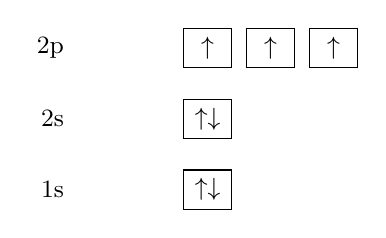
\begin{tikzpicture}[font=\small]
\def\xlab{-1.2}
\coordinate (y1) at (0,0); % 1s
\coordinate (y2) at (0,0.9); % 2s
\coordinate (y3) at (0,1.8); % 2p
% 1s
\node[left] at ($(y1)+(\xlab,0)$){1s};
\draw ($(y1)+(0.2,-0.25)$) rectangle ($(y1)+(0.8,0.25)$);
\node at ($(y1)+(0.5,0)$){$\uparrow\downarrow$};
% 2s
\node[left] at ($(y2)+(\xlab,0)$){2s};
\draw ($(y2)+(0.2,-0.25)$) rectangle ($(y2)+(0.8,0.25)$);
\node at ($(y2)+(0.5,0)$){$\uparrow\downarrow$};
% 2p (three orbitals)
\node[left] at ($(y3)+(\xlab,0)$){2p};
\foreach \i/\arr in {0/$\uparrow$,1/$\uparrow$,2/$\uparrow$}{
    \draw ($(y3)+(0.2+0.8*\i,-0.25)$) rectangle ($(y3)+(0.8+0.8*\i,0.25)$);
    \node at ($(y3)+(0.5+0.8*\i,0)$){\arr};
}
\end{tikzpicture}
\textbf{Answer:} 1s$^2$ 2s$^2$ 2p$^4$; 2 unpaired electrons in 2p orbitals.
\end{minipage}

\\
\hline
\end{tabular}

\newpage
\noindent
{\large\textbf{Content (fully worked out problems \& answers) continued...}}\\[0.2em]
\vspace{0.2cm}
\begin{tabular}{|p{0.9\linewidth}|}
\hline
\vspace{0.2cm}
\textbf{(25)} Draw the electron diagram (orbital boxes) for the chloride ion, Cl\(^{-}\). Place arrows (↑, ↓) to indicate electrons. 
\vspace{0.2cm}

\textbf{Empty orbital diagram (TikZ)}
\vspace{0.2cm}

\begin{tikzpicture}[font=\small]
  \def\xlab{-1.2}
  \coordinate (y1) at (0,0);   % 1s
  \coordinate (y2) at (0,0.9); % 2s
  \coordinate (y3) at (0,1.8); % 2p
  \coordinate (y4) at (0,2.7); % 3s
  \coordinate (y5) at (0,3.6); % 3p (three orbitals)
  % 1s
  \node[left] at ($(y1)+(\xlab,0)$){1s};
  \draw ($(y1)+(0.2,-0.25)$) rectangle ($(y1)+(0.8,0.25)$);
  % 2s
  \node[left] at ($(y2)+(\xlab,0)$){2s};
  \draw ($(y2)+(0.2,-0.25)$) rectangle ($(y2)+(0.8,0.25)$);
  % 2p (three)
  \node[left] at ($(y3)+(\xlab,0)$){2p};
  \foreach \i in {0,1,2}{
    \draw ($(y3)+(0.2+0.8*\i,-0.25)$) rectangle ($(y3)+(0.8+0.8*\i,0.25)$);
  }
  % 3s
  \node[left] at ($(y4)+(\xlab,0)$){3s};
  \draw ($(y4)+(0.2,-0.25)$) rectangle ($(y4)+(0.8,0.25)$);
  % 3p (three)
  \node[left] at ($(y5)+(\xlab,0)$){3p};
  \foreach \i in {0,1,2}{
    \draw ($(y5)+(0.2+0.8*\i,-0.25)$) rectangle ($(y5)+(0.8+0.8*\i,0.25)$);
  }
\end{tikzpicture} \\
\hline
\vspace{0.2cm}
\textbf{Solution:} Electron configuration 1s$^2$ 2s$^2$ 2p$^6$ 3s$^2$ 3p$^6$. All orbitals fully filled:
\vspace{0.2cm}

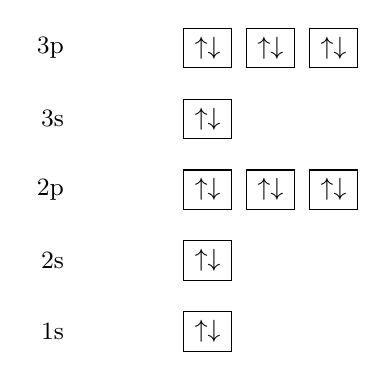
\begin{tikzpicture}[font=\small]
\def\xlab{-1.2}
\coordinate (y1) at (0,0); \coordinate (y2) at (0,0.9); \coordinate (y3) at (0,1.8);
\coordinate (y4) at (0,2.7); \coordinate (y5) at (0,3.6);
% 1s
\node[left] at ($(y1)+(\xlab,0)$){1s};
\draw ($(y1)+(0.2,-0.25)$) rectangle ($(y1)+(0.8,0.25)$); \node at ($(y1)+(0.5,0)$){$\uparrow\downarrow$};
% 2s
\node[left] at ($(y2)+(\xlab,0)$){2s};
\draw ($(y2)+(0.2,-0.25)$) rectangle ($(y2)+(0.8,0.25)$); \node at ($(y2)+(0.5,0)$){$\uparrow\downarrow$};
% 2p
\node[left] at ($(y3)+(\xlab,0)$){2p};
\foreach \i in {0,1,2}{\draw ($(y3)+(0.2+0.8*\i,-0.25)$) rectangle ($(y3)+(0.8+0.8*\i,0.25)$);
\node at ($(y3)+(0.5+0.8*\i,0)$){$\uparrow\downarrow$};}
% 3s
\node[left] at ($(y4)+(\xlab,0)$){3s};
\draw ($(y4)+(0.2,-0.25)$) rectangle ($(y4)+(0.8,0.25)$); \node at ($(y4)+(0.5,0)$){$\uparrow\downarrow$};
% 3p
\node[left] at ($(y5)+(\xlab,0)$){3p};
\foreach \i in {0,1,2}{\draw ($(y5)+(0.2+0.8*\i,-0.25)$) rectangle ($(y5)+(0.8+0.8*\i,0.25)$);
\node at ($(y5)+(0.5+0.8*\i,0)$){$\uparrow\downarrow$};}
\end{tikzpicture}
\vspace{0.2cm}
\textbf{Answer:} Fully filled orbitals; closed shell.
\vspace{0.2cm}
\\
\hline
\end{tabular}


\newpage
\noindent
{\large\textbf{Content (fully worked out problems \& answers) continued...}}\\[0.2em]
\vspace{0.2cm}
\begin{tabular}{|p{0.9\linewidth}|}
\hline
\vspace{0.2cm}
\textbf{(26)} Draw the electron diagram (orbital boxes) for neutral iron (Fe). Place arrows (↑, ↓) to indicate electrons. Use Aufbau, Hund, and Pauli. Pay attention to how 4s and 3d are filled and later how electrons are paired/unpaired in 3d.
\vspace{0.2cm}

\textbf{Empty orbital diagram (TikZ)}
\vspace{0.2cm}

\begin{tikzpicture}[font=\small]
  \def\xlab{-1.3}
  % y positions
  \coordinate (y1) at (0,0);    % 1s
  \coordinate (y2) at (0,0.8);  % 2s
  \coordinate (y3) at (0,1.6);  % 2p
  \coordinate (y4) at (0,2.4);  % 3s
  \coordinate (y5) at (0,3.2);  % 3p
  \coordinate (y6) at (0,4.0);  % 4s
  \coordinate (y7) at (0,4.8);  % 3d (five orbitals)
  % 1s
  \node[left] at ($(y1)+(\xlab,0)$){1s};
  \draw ($(y1)+(0.2,-0.22)$) rectangle ($(y1)+(0.8,0.22)$);
  % 2s
  \node[left] at ($(y2)+(\xlab,0)$){2s};
  \draw ($(y2)+(0.2,-0.22)$) rectangle ($(y2)+(0.8,0.22)$);
  % 2p
  \node[left] at ($(y3)+(\xlab,0)$){2p};
  \foreach \i in {0,1,2}{
    \draw ($(y3)+(0.2+0.8*\i,-0.22)$) rectangle ($(y3)+(0.8+0.8*\i,0.22)$);
  }
  % 3s
  \node[left] at ($(y4)+(\xlab,0)$){3s};
  \draw ($(y4)+(0.2,-0.22)$) rectangle ($(y4)+(0.8,0.22)$);
  % 3p
  \node[left] at ($(y5)+(\xlab,0)$){3p};
  \foreach \i in {0,1,2}{
    \draw ($(y5)+(0.2+0.8*\i,-0.22)$) rectangle ($(y5)+(0.8+0.8*\i,0.22)$);
  }
  % 4s
  \node[left] at ($(y6)+(\xlab,0)$){4s};
  \draw ($(y6)+(0.2,-0.22)$) rectangle ($(y6)+(0.8,0.22)$);
  % 3d (five orbitals)
  \node[left] at ($(y7)+(\xlab,0)$){3d};
  \foreach \i in {0,1,2,3,4}{
    \draw ($(y7)+(0.2+0.6*\i,-0.22)$) rectangle ($(y7)+(0.6+0.6*\i,0.22)$);
  }
\end{tikzpicture} \\
\hline
\vspace{0.2cm}

\textbf{Solution:} 1s$^2$ 2s$^2$ 2p$^6$ 3s$^2$ 3p$^6$ 4s$^2$ 3d$^6$:
\vspace{0.2cm}

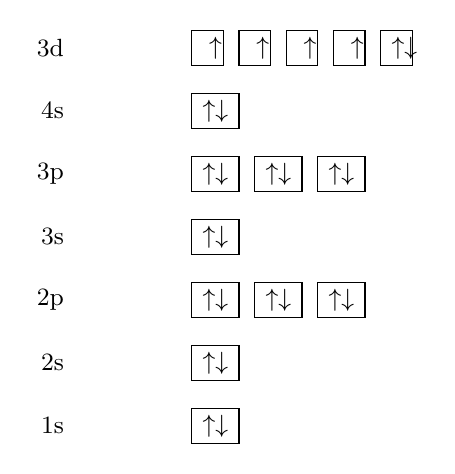
\begin{tikzpicture}[font=\small]
\def\xlab{-1.3}
\coordinate (y1) at (0,0); \coordinate (y2) at (0,0.8); \coordinate (y3) at (0,1.6);
\coordinate (y4) at (0,2.4); \coordinate (y5) at (0,3.2); \coordinate (y6) at (0,4.0); \coordinate (y7) at (0,4.8);
% 1s
\node[left] at ($(y1)+(\xlab,0)$){1s}; \draw ($(y1)+(0.2,-0.22)$) rectangle ($(y1)+(0.8,0.22)$); \node at ($(y1)+(0.5,0)$){$\uparrow\downarrow$};
% 2s
\node[left] at ($(y2)+(\xlab,0)$){2s}; \draw ($(y2)+(0.2,-0.22)$) rectangle ($(y2)+(0.8,0.22)$); \node at ($(y2)+(0.5,0)$){$\uparrow\downarrow$};
% 2p
\node[left] at ($(y3)+(\xlab,0)$){2p}; \foreach \i in {0,1,2}{\draw ($(y3)+(0.2+0.8*\i,-0.22)$) rectangle ($(y3)+(0.8+0.8*\i,0.22)$); \node at ($(y3)+(0.5+0.8*\i,0)$){$\uparrow\downarrow$};}
% 3s
\node[left] at ($(y4)+(\xlab,0)$){3s}; \draw ($(y4)+(0.2,-0.22)$) rectangle ($(y4)+(0.8,0.22)$); \node at ($(y4)+(0.5,0)$){$\uparrow\downarrow$};
% 3p
\node[left] at ($(y5)+(\xlab,0)$){3p}; \foreach \i in {0,1,2}{\draw ($(y5)+(0.2+0.8*\i,-0.22)$) rectangle ($(y5)+(0.8+0.8*\i,0.22)$); \node at ($(y5)+(0.5+0.8*\i,0)$){$\uparrow\downarrow$};}
% 4s
\node[left] at ($(y6)+(\xlab,0)$){4s}; \draw ($(y6)+(0.2,-0.22)$) rectangle ($(y6)+(0.8,0.22)$); \node at ($(y6)+(0.5,0)$){$\uparrow\downarrow$};
% 3d
\node[left] at ($(y7)+(\xlab,0)$){3d};
\foreach \i/\arr in {0/$\uparrow$,1/$\uparrow$,2/$\uparrow$,3/$\uparrow$,4/$\uparrow\downarrow$}{\draw ($(y7)+(0.2+0.6*\i,-0.22)$) rectangle ($(y7)+(0.6+0.6*\i,0.22)$); \node at ($(y7)+(0.5+0.6*\i,0)$){\arr};}
\end{tikzpicture}
\vspace{0.2cm}

\textbf{Answer:} 4 unpaired electrons in 3d.
\vspace{0.2cm}
\\
\hline
\end{tabular}


\newpage
\noindent
{\large\textbf{Content (fully worked out problems \& answers) continued...}}\\[0.2em]
\vspace{0.2cm}
\begin{tabular}{|p{0.9\linewidth}|}
\hline
\vspace{0.2cm}
\textbf{(27)} Draw the electron diagram (orbital boxes) for neutral copper (Cu). Place arrows (↑, ↓) to indicate electrons.
\vspace{0.2cm}

\textbf{Empty orbital diagram (TikZ)}
\vspace{0.2cm}

\begin{tikzpicture}[font=\small]
  \def\xlab{-1.3}
  \coordinate (y1) at (0,0);   % 1s
  \coordinate (y2) at (0,0.8); % 2s
  \coordinate (y3) at (0,1.6); % 2p
  \coordinate (y4) at (0,2.4); % 3s
  \coordinate (y5) at (0,3.2); % 3p
  \coordinate (y6) at (0,4.0); % 4s
  \coordinate (y7) at (0,4.8); % 3d (five)
  % 1s
  \node[left] at ($(y1)+(\xlab,0)$){1s};
  \draw ($(y1)+(0.2,-0.22)$) rectangle ($(y1)+(0.8,0.22)$);
  % 2s
  \node[left] at ($(y2)+(\xlab,0)$){2s};
  \draw ($(y2)+(0.2,-0.22)$) rectangle ($(y2)+(0.8,0.22)$);
  % 2p
  \node[left] at ($(y3)+(\xlab,0)$){2p};
  \foreach \i in {0,1,2}{
    \draw ($(y3)+(0.2+0.8*\i,-0.22)$) rectangle ($(y3)+(0.8+0.8*\i,0.22)$);
  }
  % 3s
  \node[left] at ($(y4)+(\xlab,0)$){3s};
  \draw ($(y4)+(0.2,-0.22)$) rectangle ($(y4)+(0.8,0.22)$);
  % 3p
  \node[left] at ($(y5)+(\xlab,0)$){3p};
  \foreach \i in {0,1,2}{
    \draw ($(y5)+(0.2+0.8*\i,-0.22)$) rectangle ($(y5)+(0.8+0.8*\i,0.22)$);
  }
  % 4s
  \node[left] at ($(y6)+(\xlab,0)$){4s};
  \draw ($(y6)+(0.2,-0.22)$) rectangle ($(y6)+(0.8,0.22)$);
  % 3d
  \node[left] at ($(y7)+(\xlab,0)$){3d};
  \foreach \i in {0,1,2,3,4}{
    \draw ($(y7)+(0.2+0.6*\i,-0.22)$) rectangle ($(y7)+(0.6+0.6*\i,0.22)$);
  }
\end{tikzpicture} \\
\hline
\vspace{0.2cm}

\textbf{Solution:} Cu has electron configuration [Ar] 3d$^{10}$ 4s$^1$:
\vspace{0.2cm}

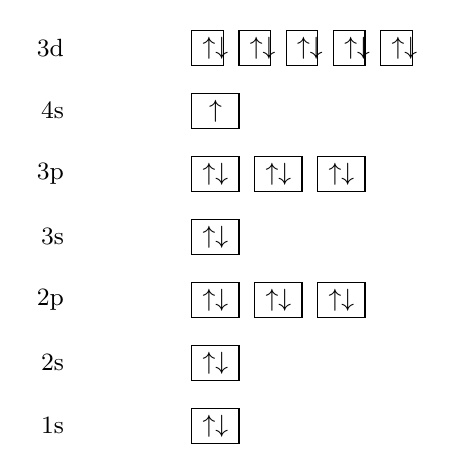
\begin{tikzpicture}[font=\small]
\def\xlab{-1.3}
\coordinate (y1) at (0,0); \coordinate (y2) at (0,0.8); \coordinate (y3) at (0,1.6);
\coordinate (y4) at (0,2.4); \coordinate (y5) at (0,3.2); \coordinate (y6) at (0,4.0); \coordinate (y7) at (0,4.8);
% 1s
\node[left] at ($(y1)+(\xlab,0)$){1s}; \draw ($(y1)+(0.2,-0.22)$) rectangle ($(y1)+(0.8,0.22)$); \node at ($(y1)+(0.5,0)$){$\uparrow\downarrow$};
% 2s
\node[left] at ($(y2)+(\xlab,0)$){2s}; \draw ($(y2)+(0.2,-0.22)$) rectangle ($(y2)+(0.8,0.22)$); \node at ($(y2)+(0.5,0)$){$\uparrow\downarrow$};
% 2p
\node[left] at ($(y3)+(\xlab,0)$){2p}; \foreach \i in {0,1,2}{\draw ($(y3)+(0.2+0.8*\i,-0.22)$) rectangle ($(y3)+(0.8+0.8*\i,0.22)$); \node at ($(y3)+(0.5+0.8*\i,0)$){$\uparrow\downarrow$};}
% 3s
\node[left] at ($(y4)+(\xlab,0)$){3s}; \draw ($(y4)+(0.2,-0.22)$) rectangle ($(y4)+(0.8,0.22)$); \node at ($(y4)+(0.5,0)$){$\uparrow\downarrow$};
% 3p
\node[left] at ($(y5)+(\xlab,0)$){3p}; \foreach \i in {0,1,2}{\draw ($(y5)+(0.2+0.8*\i,-0.22)$) rectangle ($(y5)+(0.8+0.8*\i,0.22)$); \node at ($(y5)+(0.5+0.8*\i,0)$){$\uparrow\downarrow$};}
% 4s
\node[left] at ($(y6)+(\xlab,0)$){4s}; \draw ($(y6)+(0.2,-0.22)$) rectangle ($(y6)+(0.8,0.22)$); \node at ($(y6)+(0.5,0)$){$\uparrow$};
% 3d
\node[left] at ($(y7)+(\xlab,0)$){3d}; \foreach \i in {0,1,2,3,4}{\draw ($(y7)+(0.2+0.6*\i,-0.22)$) rectangle ($(y7)+(0.6+0.6*\i,0.22)$); \node at ($(y7)+(0.5+0.6*\i,0)$){$\uparrow\downarrow$};}
\end{tikzpicture}
\vspace{0.2cm}

\textbf{Answer:} 4s$^1$ 3d$^{10}$; 1 unpaired electron in 4s.
\vspace{0.2cm}
\\
\hline
\end{tabular}

\newpage
\noindent
{\large\textbf{Content (fully worked out problems \& answers) continued...}}\\[0.2em]
\vspace{0.2cm}

\begin{tabular}{|p{0.9\linewidth}|}
\hline
\vspace{0.2cm}
\textbf{(28)} Draw the electron diagram (orbital boxes) for the sulfide ion, S\(^{2-}\). Place arrows (↑, ↓) to indicate electrons. Place arrows consistent with Aufbau, Hund, and Pauli.
\vspace{0.2cm}

\textbf{Empty orbital diagram (TikZ)}
\vspace{0.2cm}

\begin{tikzpicture}[font=\small]
  \def\xlab{-1.2}
  \coordinate (y1) at (0,0);   % 1s
  \coordinate (y2) at (0,0.9); % 2s
  \coordinate (y3) at (0,1.8); % 2p
  \coordinate (y4) at (0,2.7); % 3s
  \coordinate (y5) at (0,3.6); % 3p
  % 1s
  \node[left] at ($(y1)+(\xlab,0)$){1s};
  \draw ($(y1)+(0.2,-0.25)$) rectangle ($(y1)+(0.8,0.25)$);
  % 2s
  \node[left] at ($(y2)+(\xlab,0)$){2s};
  \draw ($(y2)+(0.2,-0.25)$) rectangle ($(y2)+(0.8,0.25)$);
  % 2p
  \node[left] at ($(y3)+(\xlab,0)$){2p};
  \foreach \i in {0,1,2}{
    \draw ($(y3)+(0.2+0.8*\i,-0.25)$) rectangle ($(y3)+(0.8+0.8*\i,0.25)$);
  }
  % 3s
  \node[left] at ($(y4)+(\xlab,0)$){3s};
  \draw ($(y4)+(0.2,-0.25)$) rectangle ($(y4)+(0.8,0.25)$);
  % 3p
  \node[left] at ($(y5)+(\xlab,0)$){3p};
  \foreach \i in {0,1,2}{
    \draw ($(y5)+(0.2+0.8*\i,-0.25)$) rectangle ($(y5)+(0.8+0.8*\i,0.25)$);
  }
  \node[anchor=west] at (3.0,1.8) {Fill: 18 electrons; closed shell is expected.};
\end{tikzpicture} \\
\hline
\vspace{0.2cm}

\textbf{Solution:} Electron configuration 1s$^2$ 2s$^2$ 2p$^6$ 3s$^2$ 3p$^6$ (like Ar):
\vspace{0.2cm}

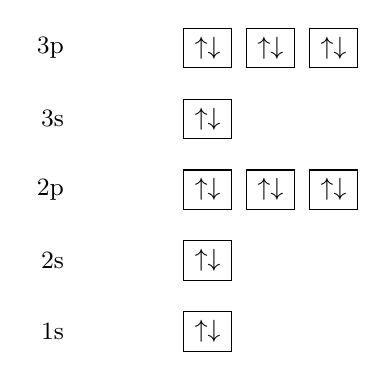
\begin{tikzpicture}[font=\small]
\def\xlab{-1.2}
\coordinate (y1) at (0,0); \coordinate (y2) at (0,0.9); \coordinate (y3) at (0,1.8);
\coordinate (y4) at (0,2.7); \coordinate (y5) at (0,3.6);
% 1s
\node[left] at ($(y1)+(\xlab,0)$){1s}; \draw ($(y1)+(0.2,-0.25)$) rectangle ($(y1)+(0.8,0.25)$); \node at ($(y1)+(0.5,0)$){$\uparrow\downarrow$};
% 2s
\node[left] at ($(y2)+(\xlab,0)$){2s}; \draw ($(y2)+(0.2,-0.25)$) rectangle ($(y2)+(0.8,0.25)$); \node at ($(y2)+(0.5,0)$){$\uparrow\downarrow$};
% 2p
\node[left] at ($(y3)+(\xlab,0)$){2p}; \foreach \i in {0,1,2}{\draw ($(y3)+(0.2+0.8*\i,-0.25)$) rectangle ($(y3)+(0.8+0.8*\i,0.25)$); \node at ($(y3)+(0.5+0.8*\i,0)$){$\uparrow\downarrow$};}
% 3s
\node[left] at ($(y4)+(\xlab,0)$){3s}; \draw ($(y4)+(0.2,-0.25)$) rectangle ($(y4)+(0.8,0.25)$); \node at ($(y4)+(0.5,0)$){$\uparrow\downarrow$};
% 3p
\node[left] at ($(y5)+(\xlab,0)$){3p}; \foreach \i in {0,1,2}{\draw ($(y5)+(0.2+0.8*\i,-0.25)$) rectangle ($(y5)+(0.8+0.8*\i,0.25)$); \node at ($(y5)+(0.5+0.8*\i,0)$){$\uparrow\downarrow$};}
\end{tikzpicture}
\vspace{0.2cm}

\textbf{Answer:} All orbitals filled; closed-shell configuration.
\vspace{0.2cm}
\\
\hline
\end{tabular}

\newpage
\noindent
{\large\textbf{Content (fully worked out problems \& answers) continued...}}\\[0.2em]
\vspace{0.2cm}
\begin{tabular}{|p{0.9\linewidth}|}
\hline
\vspace{0.2cm}
\textbf{(29)} A tectonic plate moves 860 km per day. What is its speed in m/s?\\
\begin{minipage}[t]{0.85\linewidth}
\begin{enumerate}[label=\alph*.]
   \item 0.995 m/s \
   \item 9.95 m/s \
   \item 95.9 m/s \
   \item 0.0959 m/s
\end{enumerate}
\end{minipage}\\
\hline
\vspace{0.2cm}
\textbf{Answer:}\\
\[
\text{Speed}=\frac{860~\cancel{\text{km}}}{\cancel{\text{day}}}\times\frac{1000~\text{m}}{1~\cancel{\text{km}}}\times\frac{1~\cancel{\text{day}}}{86400~\text{s}}=9.95~\text{m/s}
\] \\
\hline
\end{tabular}

\newpage
\noindent
{\large\textbf{Content (fully worked out problems \& answers) continued...}}\\[0.2em]
\vspace{0.2cm}
\begin{tabular}{|p{0.9\linewidth}|}
\hline
\vspace{0.2cm}
\textbf{(30)} Convert 750 mL to $\text{in}^3$. (Use $1~\text{in}=2.54~\text{cm}$)\\
\begin{minipage}[t]{0.85\linewidth}
\begin{enumerate}[label=\alph*.]
   \item 4.58 $\text{in}^3$ \
   \item 45.8 $\text{in}^3$ \
   \item 458 $\text{in}^3$ \
   \item 0.458 $\text{in}^3$
\end{enumerate}
\end{minipage}\\
\hline
\vspace{0.2cm}
\textbf{Answer:}\\
\[
750~\text{mL}=750~\text{cm}^3,\quad 1~\text{in}^3=(2.54~\text{cm})^3=16.387~\text{cm}^3
\]
\[
\text{Volume}=\frac{750~\text{cm}^3}{16.387~\text{cm}^3/\text{in}^3}=45.8~\text{in}^3
\] \\
\hline
\end{tabular}

\newpage
\noindent
{\large\textbf{Content (fully worked out problems \& answers) continued...}}\\[0.2em]
\vspace{0.2cm}
\begin{tabular}{|p{0.9\linewidth}|}
\hline
\vspace{0.2cm}
\textbf{(31)} Convert 88.0 kPa to atm. (Use $1~\text{atm}=101.325~\text{kPa}$)\\
\begin{minipage}[t]{0.85\linewidth}
\begin{enumerate}[label=\alph*.]
   \item 0.868 atm \
   \item 0.880 atm \
   \item 1.15 atm \
   \item 0.815 atm
\end{enumerate}
\end{minipage}\\
\hline
\vspace{0.2cm}
\textbf{Answer:}\\
\[
\text{Pressure}=\frac{88.0~\cancel{\text{kPa}}}{1}\times\frac{1~\text{atm}}{101.325~\cancel{\text{kPa}}}=0.868~\text{atm}
\] \\
\hline
\end{tabular}

\newpage
\noindent
{\large\textbf{Content (fully worked out problems \& answers) continued...}}\\[0.2em]
\vspace{0.2cm}
\begin{tabular}{|p{0.9\linewidth}|}
\hline
\vspace{0.2cm}
\textbf{(32)} Convert 4.6 g/L to mg/dL.\\
\begin{minipage}[t]{0.85\linewidth}
\begin{enumerate}[label=\alph*.]
   \item 0.46 mg/dL \
   \item 4.6 mg/dL \
   \item 46 mg/dL \
   \item 460 mg/dL
\end{enumerate}
\end{minipage}\\
\hline
\vspace{0.2cm}
\textbf{Answer:}\\
\[
\frac{4.6~\cancel{\text{g}}}{\cancel{\text{L}}}\times\frac{1000~\text{mg}}{1~\cancel{\text{g}}}\times\frac{1~\text{dL}}{10~\cancel{\text{L}}}=46~\text{mg/dL}
\] \\
\hline
\end{tabular}

\newpage
\noindent
{\large\textbf{Content (fully worked out problems \& answers) continued...}}\\[0.2em]
\vspace{0.2cm}
\begin{tabular}{|p{0.9\linewidth}|}
\hline
\vspace{0.2cm}
\textbf{(33)} A block has mass 245.0 g and dimensions 4.50 cm $\times$ 3.20 cm $\times$ 2.10 cm. Find its density in kg/m$^3$.\\
\begin{minipage}[t]{0.85\linewidth}
\begin{enumerate}[label=\alph*.]
   \item $8.10\times10^{2}~\text{kg/m}^3$ \
   \item $8.10\times10^{3}~\text{kg/m}^3$ \
   \item $8.10\times10^{4}~\text{kg/m}^3$ \
   \item $8.10\times10^{5}~\text{kg/m}^3$
\end{enumerate}
\end{minipage}\\
\hline
\vspace{0.2cm}
\textbf{Answer:}\\
\[
V=(4.50)(3.20)(2.10)~\text{cm}^3=30.2~\text{cm}^3
\]
\[
\rho=\frac{245.0~\text{g}}{30.2~\text{cm}^3}=8.10~\text{g/mL}=8.10~\frac{\text{g}}{\text{cm}^3}
\]
\[
\text{Density}=\left(8.10~\frac{\text{g}}{\text{cm}^3}\right)\times\frac{1~\text{kg}}{1000~\text{g}}\times\frac{10^6~\text{cm}^3}{1~\text{m}^3}=8.10\times10^{3}~\text{kg/m}^3
\] \\
\hline
\end{tabular}

\newpage
\noindent
{\large\textbf{Content (fully worked out problems \& answers) continued...}}\\
\vspace{0.2cm}
\begin{tabular}{|p{0.9\linewidth}|}
\hline
\vspace{0.2cm}
\textbf{(34)} A 0.500 g sample of NaCl dissolves in 250.0 mL of water. What is the concentration in g/L?\\
\hline
\vspace{0.2cm}
\begin{minipage}[t]{0.85\linewidth}
\begin{enumerate}[label=\alph*.]
\item 0.125 g/L \
\item 2.00 g/L  \
\item 1.25 g/L \
\item 0.250 g/L
\end{enumerate}
\end{minipage} \\
\hline
\vspace{0.2cm}
\textbf{Answer:} 
\[
\text{Concentration} = \frac{0.500~\text{g}}{0.250~\text{L}} = 2.00~\text{g/L}
\] \\
\\
\hline
\end{tabular}

\newpage
\noindent
{\large\textbf{Content (fully worked out problems \& answers) continued...}}\\[0.2em]
\vspace{0.2cm}
\begin{tabular}{|p{0.9\linewidth}|}
\hline
\vspace{0.2cm}
\textbf{(35)} Convert 987.0 mbar to Pa.\\
\hline
\vspace{0.2cm}
\begin{minipage}[t]{0.85\linewidth}
\begin{enumerate}[label=\alph*.]
\item 9.870 Pa \
\item 9.87 $\times$ 10$^2$ Pa \
\item 9.87 $\times$ 10$^4$ Pa \
\item 9.87 $\times$ 10$^5$ Pa
\end{enumerate}
\end{minipage} \\
\hline
\vspace{0.2cm}
\textbf{Answer:} 
\[
987.0~\text{mbar} \times \frac{100~\text{Pa}}{1~\text{mbar}} = 9.870 \times 10^4~\text{Pa}
\] \\ 
\hline
\end{tabular}

\newpage
\noindent
{\large\textbf{Content (fully worked out problems \& answers) continued...}}\\[0.2em]
\vspace{0.2cm}
\begin{tabular}{|p{0.9\linewidth}|}
\hline
\vspace{0.2cm}
\textbf{(36)} A sample occupies 250.0 mL and has a mass of 0.890 g. Calculate its density.\\
\hline
\vspace{0.2cm}
\begin{minipage}[t]{0.85\linewidth}
\begin{enumerate}[label=\alph*.]
\item 3.56 \times $10^{-3}$ g/mL \
\item 0.890 g/mL \
\item 3.56 g/mL \
\item 35.6 g/mL
\end{enumerate}
\end{minipage}\\
\hline
\vspace{0.2cm}
\textbf{Answer:} 
\[
\rho = \frac{0.890~\text{g}}{250.0~\text{mL}} = 3.56 \times 10^{-3}~\text{g/mL}
\] \\ 
\hline
\end{tabular}

\newpage
\noindent
{\large\textbf{Content (fully worked out problems \& answers) continued...}}\\[0.2em]
\vspace{0.2cm}
\begin{tabular}{|p{0.9\linewidth}|}
\hline
\vspace{0.2cm}
\textbf{(37)} A beaker contains 3.50 L of solution. Express this volume in cubic decimeters (dm$^3$) using unit factors.\\
\hline
\vspace{0.2cm}
\begin{minipage}[t]{0.85\linewidth}
\begin{enumerate}[label=\alph*.]
\item 0.00350 dm$^3$ \
\item 3.50 dm$^3$ \
\item 35.0 dm$^3$ \
\item 350 dm$^3$
\end{enumerate}
\end{minipage} \\
\hline
\vspace{0.2cm}
\textbf{Answer:} 
\[
3.50~\text{L} \times \frac{{10^{-3}}~\text{dm}^3}{1~\text{L}} = 0.00350~\text{dm}^3
\] \\
\hline
\end{tabular}

\newpage
\noindent
{\large\textbf{Content (fully worked out problems \& answers) continued...}}\\[0.2em]
\vspace{0.2cm}
\begin{tabular}{|p{0.9\linewidth}|}
\hline
\vspace{0.2cm}
\textbf{(38)} A student measures 0.00250 kg of a substance. Express this in grams.\\
\hline
\vspace{0.2cm}
\begin{minipage}[t]{0.85\linewidth}
\begin{enumerate}[label=\alph*.]
\item 0.00250 g \
\item 0.0250 g \
\item 2.50 g \
\item 250 g 
\end{enumerate}
\end{minipage}\\
\hline
\vspace{0.2cm}
\textbf{Answer:} 
\[
0.00250~\text{kg} \times \frac{1000~\text{g}}{1~\text{kg}} = 2.50~\text{g}
\] \\ 
\hline
\end{tabular}

\newpage
\noindent
{\large\textbf{Content (fully worked out problems \& answers) continued...}}\\[0.2em]
\vspace{0.2cm}
\begin{tabular}{|p{0.9\linewidth}|}
\hline
\vspace{0.2cm}
\textbf{(39)} A 5.00 mL sample of water weighs 4.98 g. What is its density?\\
\hline
\vspace{0.2cm}
\begin{minipage}[t]{0.85\linewidth}
\begin{enumerate}[label=\alph*.]
\item 0.996 g/mL \
\item 1.00 g/mL \
\item 1.02 g/mL \ 
\item 1.10 g/mL 
\end{enumerate}
\end{minipage}\\
\hline
\vspace{0.2cm}
\textbf{Answer:} 
\[
\rho = \frac{4.98~\text{g}}{5.00~\text{mL}} = 0.996~\text{g/mL}
\] \\ 
\hline
\end{tabular}
\newpage

\noindent
{\large\textbf{Content (fully worked out problems \& answers) continued...}}\\[0.2em]
\vspace{0.2cm}
\begin{tabular}{|p{0.9\linewidth}|}
\hline
\vspace{0.2cm}
\textbf{(40)} Which of the following is an isotope of carbon? \\
\begin{minipage}[t]{0.85\linewidth}
\begin{enumerate}[label=\alph*.]
\item $^{12}$C \
\item $^{14}$C \
\item Both a and b \ 
\item $^{16}$O 
\end{enumerate}
\end{minipage}\\
\hline
\vspace{0.2cm}
\textbf{Solution:} \\
Isotopes are atoms of the same element with different mass numbers (different neutrons). Both $^{12}$C and $^{14}$C are carbon isotopes. \\
\hline
\vspace{0.2cm}
\textbf{Answer:} c. Both a and b \\
\hline
\end{tabular}
\newpage

\noindent
{\large\textbf{Content (fully worked out problems \& answers) continued...}}\\[0.2em]
\vspace{0.2cm}
\begin{tabular}{|p{0.9\linewidth}|}
\hline
\vspace{0.2cm}
\textbf{(41)} Which subatomic particle determines the identity of an element? \\
\begin{minipage}[t]{0.85\linewidth}
\begin{enumerate}[label=\alph*.]
\item Proton \
\item Electron \
\item Neutron \
\item Nucleus \
\end{enumerate}
\end{minipage}\\
\hline
\vspace{0.2cm}
\textbf{Solution:} \\
The number of protons (atomic number) defines the element. Changing the number of protons changes the element. \\
\hline
\vspace{0.2cm}
\textbf{Answer:} a. Proton \\
\hline
\end{tabular}
\newpage

\noindent
{\large\textbf{Content (fully worked out problems \& answers) continued...}}\\[0.2em]
\vspace{0.2cm}
\begin{tabular}{|p{0.9\linewidth}|}
\hline
\vspace{0.2cm}
\textbf{(42)} An atom of sodium (Na) loses one electron. What is the resulting ion? \\
\begin{minipage}[t]{0.85\linewidth}
\begin{enumerate}[label=\alph*.]
\item Na$^-$ \
\item Na$^{+}$ \
\item Na$^{2+}$ \
\item Neutral Na
\end{enumerate}
\end{minipage}\\
\hline
\vspace{0.2cm}
\textbf{Solution:} \\
Losing one electron creates a positive charge. Sodium forms Na$^{+}$ when it loses one electron. \\
\hline
\vspace{0.2cm}
\textbf{Answer:} b. Na$^{+}$ \\
\hline
\end{tabular}
\newpage

\noindent
{\large\textbf{Content (fully worked out problems \& answers) continued...}}\\[0.2em]
\vspace{0.2cm}
\begin{tabular}{|p{0.9\linewidth}|}
\hline
\vspace{0.2cm}
\textbf{(43)} Which of the following are isotopes of the same element? \\
\begin{minipage}[t]{0.85\linewidth}
\begin{enumerate}[label=\alph*.]
\item $^{1}$H and $^{2}$H \
\item $^{12}$C and $^{14}$N \
\item $^{16}$O and $^{18}$F \
\item $^{23}$Na and $^{24}$Mg
\end{enumerate}
\end{minipage}\\
\hline
\vspace{0.2cm}
\textbf{Solution:} \\
Isotopes are atoms with the same number of protons but different neutrons. $^{1}$H and $^{2}$H are hydrogen isotopes. \\
\hline
\vspace{0.2cm}
\textbf{Answer:} a. $^{1}$H and $^{2}$H \\
\hline
\end{tabular}

\newpage

\noindent
{\large\textbf{Content (fully worked out problems \& answers) continued...}}\\[0.2em]
\vspace{0.2cm}
\begin{tabular}{|p{0.9\linewidth}|}
\hline
\vspace{0.2cm}
\textbf{(46)} Which type of bond is expected between Na and Cl in NaCl? \\
\begin{minipage}[t]{0.85\linewidth}
\begin{enumerate}[label=\alph*.]
\item Nonpolar covalent \
\item Polar covalent \
\item Ionic \
\item Metallic
\end{enumerate}
\end{minipage}\\
\hline
\vspace{0.2cm}
\textbf{Solution:} \\
Electronegativity difference between Na (0.9) and Cl (3.0) is about 2.1, which is large. A difference greater than $\sim 2.0$ typically indicates ionic bonding. Thus, Na transfers an electron to Cl, forming an ionic bond. \\
\hline
\vspace{0.2cm}
\textbf{Answer:} c. Ionic \\
\hline
\end{tabular}
\newpage

\noindent
{\large\textbf{Content (fully worked out problems \& answers) continued...}}\\[0.2em]
\vspace{0.2cm}
\begin{tabular}{|p{0.9\linewidth}|}
\hline
\vspace{0.2cm}
\textbf{(47)} Which of the following has the highest electronegativity? \\
\begin{minipage}[t]{0.85\linewidth}
\begin{enumerate}[label=\alph*.]
\item Lithium \
\item Carbon \
\item Fluorine \
\item Oxygen
\end{enumerate}
\end{minipage}\\
\hline
\vspace{0.2cm}
\textbf{Solution:} \\
Electronegativity increases across a period and decreases down a group. Fluorine is the most electronegative element (value $\approx 4.0$), higher than oxygen (3.5), carbon (2.5), and lithium (1.0). \\
\hline
\vspace{0.2cm}
\textbf{Answer:} c. Fluorine \\
\hline
\end{tabular}
\newpage

\noindent
{\large\textbf{Content (fully worked out problems & answers) continued...}}\\[0.2em]
\vspace{0.2cm}
\begin{tabular}{|p{0.9\linewidth}|}
\hline
\vspace{0.2cm}
\textbf{(48)} What is the correct name for $\text{MgF}_2$? \\
\begin{minipage}[t]{0.85\linewidth}
\begin{enumerate}[label=\alph*.]
\item Magnesium difluoride \
\item Magnesium fluoride \
\item Magnesium(II) fluoride \
\item Monomagnesium fluoride
\end{enumerate}
\end{minipage}\\
\hline
\vspace{0.2cm}
\textbf{Solution:} \\
Magnesium is Group 2 (+2). Fluoride is -1, two are needed to balance. The correct name is magnesium fluoride. \\
\hline
\vspace{0.2cm}
\textbf{Answer:} b. Magnesium fluoride \
\hline
\end{tabular}

\newpage
\noindent
{\large\textbf{Content (fully worked out problems \& answers) continued...}}\\[0.2em]
\vspace{0.2cm}
\begin{tabular}{|p{0.9\linewidth}|}
\hline
\vspace{0.2cm}
\textbf{(49)} Which is the correct name for $\text{Cu}_2\text{O}$? \\
\begin{minipage}[t]{0.85\linewidth}
\begin{enumerate}[label=\alph*.]
\item Copper(I) oxide \
\item Copper(II) oxide \
\item Dicopper monoxide \
\item Copper oxide
\end{enumerate}
\end{minipage}\\
\hline
\vspace{0.2cm}
\textbf{Solution:} \\
Oxygen is -2. Two Cu atoms balance it, so each Cu is +1. Correct name: Copper(I) oxide. \\
\hline
\vspace{0.2cm}
\textbf{Answer:} a. Copper(I) oxide \
\hline
\end{tabular}

\newpage
\noindent
{\large\textbf{Content (fully worked out problems \& answers) continued...}}\\[0.2em]

\begin{tabular}{|p{0.9\linewidth}|}
\hline
\vspace{0.2cm}
\textbf{(50)} What is the formula for lithium sulfide? \\
\begin{minipage}[t]{0.85\linewidth}
\begin{enumerate}[label=\alph*.]
\item LiS \\
\item Li$_2$S \\
\item LiS$_2$ \\
\item Li$_2$S$_3$
\end{enumerate}
\end{minipage}\\
\hline
\vspace{0.2cm}
\textbf{Solution:} \\
Lithium is +1, sulfide is -2. Two Li$^{+}$ are required for one S$^{2-}$. Formula: Li$_2$S. \\
\hline
\vspace{0.2cm}
\textbf{Answer:} b. Li$_2$S \\
\hline
\end{tabular}


\newpage
\noindent
{\large\textbf{Content (fully worked out problems \& answers) continued...}}\\[0.2em]

\begin{tabular}{|p{0.9\linewidth}|}
\hline
\vspace{0.2cm}
\textbf{(51)} What is the correct name for $\text{PbO}_2$? \\
\begin{minipage}[t]{0.85\linewidth}
\begin{enumerate}[label=\alph*.]
\item Lead(II) oxide \
\item Lead(IV) oxide \
\item Lead oxide \
\item Dilead dioxide
\end{enumerate}
\end{minipage}\\
\hline
\vspace{0.2cm}
\textbf{Solution:} \\
Oxygen is -2, two atoms total -4. Pb must be +4. Correct name: Lead(IV) oxide. \\
\hline
\vspace{0.2cm}
\textbf{Answer:} b. Lead(IV) oxide \
\hline
\end{tabular}

\newpage
\noindent
{\large\textbf{Content (fully worked out problems \& answers) continued...}}\\[0.2em]

\begin{tabular}{|p{0.9\linewidth}|}
\hline
\vspace{0.2cm}
\textbf{(52)} Which of the following is the correct formula for strontium chloride? \\
\begin{minipage}[t]{0.85\linewidth}
\begin{enumerate}[label=\alph*.]
\item SrCl \\
\item Sr$_2$Cl \\
\item SrCl$_2$ \\
\item Sr$_2$Cl$_3$
\end{enumerate}
\end{minipage}\\
\hline
\vspace{0.2cm}
\textbf{Solution:} \\
Strontium is Group 2 (+2). Chloride is -1, so two Cl$^{-}$ are needed. Formula: SrCl$_2$. \\
\hline
\vspace{0.2cm}
\textbf{Answer:} c. SrCl$_2$ \\
\hline
\end{tabular}
\newpage
\noindent
{\large\textbf{Content (fully worked out problems & answers) continued...}}\\[0.2em]
\vspace{0.2cm}
\begin{tabular}{|p{0.9\linewidth}|}
\hline
\vspace{0.2cm}
\textbf{(53)} What is the correct name for $\text{FeCl}_3$? \\
\begin{minipage}[t]{0.85\linewidth}
\begin{enumerate}[label=\alph*.]
\item Iron chloride \
\item Iron(II) chloride \
\item Iron(III) chloride \
\item Ferrous chloride
\end{enumerate}
\end{minipage}\\
\hline
\vspace{0.2cm}
\textbf{Solution:} \\
Each Cl is -1, three Cl give -3 total, so Fe must be +3. Use Roman numeral: Iron(III) chloride. \\
\hline
\vspace{0.2cm}
\textbf{Answer:} c. Iron(III) chloride \
\hline
\end{tabular}

\newpage
\noindent
{\large\textbf{Content (fully worked out problems \& answers) continued...}}\\[0.2em]

\begin{tabular}{|p{0.9\linewidth}|}
\hline
\vspace{0.2cm}
\textbf{(54)} Which is the correct name for $\text{CoO}$? \\
\begin{minipage}[t]{0.85\linewidth}
\begin{enumerate}[label=\alph*.]
\item Cobalt oxide \
\item Cobalt(II) oxide \
\item Cobalt(III) oxide \
\item Dicobalt monoxide
\end{enumerate}
\end{minipage}\\
\hline
\vspace{0.2cm}
\textbf{Solution:} \\
O is -2, one Co balances with +2. That gives cobalt in the +2 oxidation state: Cobalt(II) oxide. \\
\hline
\vspace{0.2cm}
\textbf{Answer:} b. Cobalt(II) oxide \
\hline
\end{tabular}

\newpage
\noindent
{\large\textbf{Content (fully worked out problems \& answers) continued...}}\\[0.2em]

\begin{tabular}{|p{0.9\linewidth}|}
\hline
\vspace{0.2cm}
\textbf{(55)} What is the correct name for $\text{Cu}_2\text{S}$? \\
\begin{minipage}[t]{0.85\linewidth}
\begin{enumerate}[label=\alph*.]
\item Copper sulfide \
\item Copper(II) sulfide \
\item Copper(I) sulfide \
\item Dicopper monosulfide
\end{enumerate}
\end{minipage}\\
\hline
\vspace{0.2cm}
\textbf{Solution:} \\
Sulfide is -2. Two Cu atoms give +2 total so each Cu is +1. Name uses Roman numeral: Copper(I) sulfide. \\
\hline
\vspace{0.2cm}
\textbf{Answer:} c. Copper(I) sulfide \
\hline
\end{tabular}

\newpage
\noindent
{\large\textbf{Content (fully worked out problems & answers) continued...}}\\[0.2em]
\begin{tabular}{|p{0.9\linewidth}|}
\hline
\vspace{0.2cm}
\textbf{(56)} What is the correct name for $\text{Zn(NO}_3)_2$? \\
\begin{minipage}[t]{0.85\linewidth}
\begin{enumerate}[label=\alph*.]
\item Zinc nitrate \
\item Zinc dinitrate \
\item Zinc(II) nitrite \
\item Zinc nitrite
\end{enumerate}
\end{minipage}\
\hline
\vspace{0.2cm}
\textbf{Solution:} Nitrate is $-1$; two nitrates give $-2$, so Zn must be $+2$. Name: zinc (common oxidation state +2) with nitrate. \
\hline
\vspace{0.2cm}
\textbf{Answer:} a. Zinc nitrate \
\hline
\end{tabular}
\newpage
\noindent
{\large\textbf{Content (fully worked out problems & answers) continued...}}\\[0.2em]
\begin{tabular}{|p{0.9\linewidth}|}
\hline
\vspace{0.2cm}
\textbf{(57)} Which is the correct formula for silver sulfate? \\
\begin{minipage}[t]{0.85\linewidth}
\begin{enumerate}[label=\alph*.]
\item AgSO$_4$ \
\item Ag$_2$SO$_4$ \
\item Ag(SO$_4$)$_2$ \
\item Ag$_2$(SO$_3$)
\end{enumerate}
\end{minipage}\
\hline
\vspace{0.2cm}
\textbf{Solution:} Sulfate is $-2$ and Ag is $+1$, so two Ag$^+$ are needed per sulfate: formula Ag$_2$SO$_4$. \
\hline
\vspace{0.2cm}
\textbf{Answer:} b. Ag$_2$SO$_4$ \
\hline
\end{tabular}
\newpage
\noindent
{\large\textbf{Content (fully worked out problems & answers) continued...}}\\[0.2em]
\begin{tabular}{|p{0.9\linewidth}|}
\hline
\vspace{0.2cm}
\textbf{(58)} What is the correct name for $\text{Cd(OH)}_2$? \\
\begin{minipage}[t]{0.85\linewidth}
\begin{enumerate}[label=\alph*.]
\item Cadmium hydroxide \
\item Cadmium(II) hydroxide \
\item Cadmium dihydroxide \
\item Cadmium(I) hydroxide
\end{enumerate}
\end{minipage}\
\hline
\vspace{0.2cm}
\textbf{Solution:} Hydroxide is $-1$; two OH$^-$ give $-2$, so Cd is $+2$. Proper systematic name: cadmium(II) hydroxide (commonly "cadmium hydroxide"). \
\hline
\vspace{0.2cm}
\textbf{Answer:} b. Cadmium(II) hydroxide \
\hline
\end{tabular}
\newpage
\noindent
{\large\textbf{Content (fully worked out problems & answers) continued...}}\\[0.2em]
\begin{tabular}{|p{0.9\linewidth}|}
\hline
\vspace{0.2cm}
\textbf{(59)} Which is the correct name for $\text{Ga}_2(\text{CO}_3)_3$? \\
\begin{minipage}[t]{0.85\linewidth}
\begin{enumerate}[label=\alph*.]
\item Gallium carbonate \
\item Gallium(II) carbonate \
\item Gallium(III) carbonate \
\item Digallium tricarbonate
\end{enumerate}
\end{minipage}\
\hline
\vspace{0.2cm}
\textbf{Solution:} Carbonate is $-2$; three give $-6$, two Ga supply $+6$ total so each Ga is $+3$. Name: gallium(III) carbonate (commonly "gallium carbonate"). \
\hline
\vspace{0.2cm}
\textbf{Answer:} c. Gallium(III) carbonate \
\hline
\end{tabular}
\newpage
\noindent
{\large\textbf{Content (fully worked out problems & answers) continued...}}\\[0.2em]
\begin{tabular}{|p{0.9\linewidth}|}
\hline
\vspace{0.2cm}
\textbf{(60)} What is the formula for ammonium phosphate? \\
\begin{minipage}[t]{0.85\linewidth}
\begin{enumerate}[label=\alph*.]
\item (NH$_4$)PO$_4$ \
\item (NH$_4$)$_2$PO$_4$ \
\item (NH$_4$)$_3$PO$_4$ \
\item NH$_4$PO$_4$
\end{enumerate}
\end{minipage}\
\hline
\vspace{0.2cm}
\textbf{Solution:} Phosphate is $-3$; ammonium is $+1$ so three NH$_4^+$ are needed to balance one PO$_4^{3-}$: (NH$_4$)$_3$PO$_4$. \
\hline
\vspace{0.2cm}
\textbf{Answer:} c. (NH$_4$)$_3$PO$_4$ \
\hline
\end{tabular}
\newpage
\noindent
{\large\textbf{Content (fully worked out problems & answers) continued...}}\\[0.2em]
\begin{tabular}{|p{0.9\linewidth}|}
\hline
\vspace{0.2cm}
\textbf{(61)} What is the correct name for $\text{Al}_2(\text{SO}_4)_3$? \\
\begin{minipage}[t]{0.85\linewidth}
\begin{enumerate}[label=\alph*.]
\item Aluminum sulfate \
\item Aluminum(III) sulfate \
\item Dialuminum trisulfate \
\item Aluminum sulfite
\end{enumerate}
\end{minipage}\
\hline
\vspace{0.2cm}
\textbf{Solution:} Sulfate is $-2$; three sulfates give $-6$, two Al give $+6$ so Al is $+3$. Common name: aluminum sulfate (aluminum(III) sulfate is equivalent). \
\hline
\vspace{0.2cm}
\textbf{Answer:} a. Aluminum sulfate \
\hline
\end{tabular}
\newpage
\noindent
{\large\textbf{Content (fully worked out problems & answers) continued...}}\\[0.2em]
\begin{tabular}{|p{0.9\linewidth}|}
\hline
\vspace{0.2cm}
\textbf{(62)} Which is the correct formula for zinc acetate? \\
\begin{minipage}[t]{0.85\linewidth}
\begin{enumerate}[label=\alph*.]
\item Zn(C$_2$H$_3$O$_2$) \
\item Zn(C$_2$H$_3$O$_2$)$_2$ \
\item Zn$_2$(C$_2$H$_3$O$_2$)$_3$ \
\item Zn$_2$(C$_2$H$_3$O$_2$)$_2$
\end{enumerate}
\end{minipage}\
\hline
\vspace{0.2cm}
\textbf{Solution:} Acetate is $-1$; Zn is $+2$, so two acetates are needed: Zn(C$_2$H$_3$O$_2$)$_2$. \
\hline
\vspace{0.2cm}
\textbf{Answer:} b. Zn(C$_2$H$_3$O$_2$)$_2$ \
\hline
\end{tabular}
\newpage
\noindent
{\large\textbf{Content (fully worked out problems & answers) continued...}}\\[0.2em]
\begin{tabular}{|p{0.9\linewidth}|}
\hline
\vspace{0.2cm}
\textbf{(63)} What is the correct name for $\text{Ag}_3(\text{PO}_4)$? \\
\begin{minipage}[t]{0.85\linewidth}
\begin{enumerate}[label=\alph*.]
\item Silver phosphate \
\item Silver(III) phosphate \
\item Trisilver phosphate \
\item Silver(I) phosphate
\end{enumerate}
\end{minipage}\
\hline
\vspace{0.2cm}
\textbf{Solution:} Phosphate is $-3$, Ag is $+1$ so three Ag$^+$ balance one PO$_4^{3-}$. Name: silver phosphate (silver(I) phosphate is equivalent). \
\hline
\vspace{0.2cm}
\textbf{Answer:} a. Silver phosphate \
\hline
\end{tabular}
\newpage
\noindent
{\large\textbf{Content (fully worked out problems & answers) continued...}}\\[0.2em]
\begin{tabular}{|p{0.9\linewidth}|}
\hline
\vspace{0.2cm}
\textbf{(64)} Which is the correct formula for cadmium sulfite? \\
\begin{minipage}[t]{0.85\linewidth}
\begin{enumerate}[label=\alph*.]
\item CdSO$_3$ \
\item Cd$_2$(SO$_3$)$_3$ \
\item Cd(SO$_3$)$_2$ \
\item Cd$_3$(SO$_3$)$_2$
\end{enumerate}
\end{minipage}\
\hline
\vspace{0.2cm}
\textbf{Solution:} Sulfite is $-2$; Cd is typically $+2$, so a 1:1 formula CdSO$_3$. \
\hline
\vspace{0.2cm}
\textbf{Answer:} a. CdSO$_3$ \
\hline
\end{tabular}
\newpage
\noindent
{\large\textbf{Content (fully worked out problems & answers) continued...}}\\[0.2em]
\begin{tabular}{|p{0.9\linewidth}|}
\hline
\vspace{0.2cm}
\textbf{(65)} What is the correct name for $\text{Ga(NO}_2)_3$? \\
\begin{minipage}[t]{0.85\linewidth}
\begin{enumerate}[label=\alph*.]
\item Gallium nitrate \
\item Gallium nitrite \
\item Gallium(III) nitrite \
\item Gallium trinitrate
\end{enumerate}
\end{minipage}\
\hline
\vspace{0.2cm}
\textbf{Solution:} Nitrite is $-1$; three nitrites give $-3$, Ga must be $+3$. Proper name: gallium(III) nitrite (commonly "gallium nitrite"). \
\hline
\vspace{0.2cm}
\textbf{Answer:} c. Gallium(III) nitrite \
\hline
\end{tabular}
\newpage
\noindent
{\large\textbf{Content (fully worked out problems & answers) continued...}}\\[0.2em]
\begin{tabular}{|p{0.9\linewidth}|}
\hline
\vspace{0.2cm}
\textbf{(66)} What is the formula for ammonium chromate? \\
\begin{minipage}[t]{0.85\linewidth}
\begin{enumerate}[label=\alph*.]
\item (NH$_4$)CrO$_4$ \
\item (NH$_4$)$_2$CrO$_4$ \
\item (NH$_4$)$_3$CrO$_4$ \
\item NH$_4$CrO$_4$
\end{enumerate}
\end{minipage}\
\hline
\vspace{0.2cm}
\textbf{Solution:} Chromate is CrO$_4^{2-}$; ammonium is $+1$, so two ammoniums are required: (NH$_4$)$_2$CrO$_4$. \
\hline
\vspace{0.2cm}
\textbf{Answer:} b. (NH$_4$)$_2$CrO$_4$ \
\hline
\end{tabular}
\newpage
\noindent
{\large\textbf{Content (fully worked out problems & answers) continued...}}\\[0.2em]
\begin{tabular}{|p{0.9\linewidth}|}
\hline
\vspace{0.2cm}
\textbf{(67)} Which is the correct name for $\text{Zn(CN)}_2$? \\
\begin{minipage}[t]{0.85\linewidth}
\begin{enumerate}[label=\alph*.]
\item Zinc cyanide \
\item Zinc dicyanide \
\item Zinc(II) cyanide \
\item Zinc cyanate
\end{enumerate}
\end{minipage}\
\hline
\vspace{0.2cm}
\textbf{Solution:} Cyanide is $-1$; two CN$^-$ balance Zn$^{2+}$ giving Zn(CN)$_2$. Name: zinc cyanide (or zinc(II) cyanide). \
\hline
\vspace{0.2cm}
\textbf{Answer:} a. Zinc cyanide \
\hline
\end{tabular}
\newpage
\noindent
{\large\textbf{Content (fully worked out problems & answers) continued...}}\\[0.2em]
\begin{tabular}{|p{0.9\linewidth}|}
\hline
\vspace{0.2cm}
\textbf{(68)} What is the correct name for $\text{Al(OH)}_3$? \\
\begin{minipage}[t]{0.85\linewidth}
\begin{enumerate}[label=\alph*.]
\item Aluminum hydroxide \
\item Aluminum(III) hydroxide \
\item Trialuminum hydroxide \
\item Aluminum dihydroxide
\end{enumerate}
\end{minipage}\
\hline
\vspace{0.2cm}
\textbf{Solution:} Hydroxide is $-1$; three OH$^-$ give $-3$, so Al is $+3$. Name: aluminum hydroxide (aluminum(III) hydroxide is explicit). \
\hline
\vspace{0.2cm}
\textbf{Answer:} a. Aluminum hydroxide \
\hline
\end{tabular}
\newpage
\noindent
{\large\textbf{Content (fully worked out problems & answers) continued...}}\\[0.2em]
\begin{tabular}{|p{0.9\linewidth}|}
\hline
\vspace{0.2cm}
\textbf{(69)} Which is the correct formula for silver acetate? \\
\begin{minipage}[t]{0.85\linewidth}
\begin{enumerate}[label=\alph*.]
\item AgC$_2$H$_3$O$_2$ \
\item Ag(C$_2$H$_3$O$_2$)$_2$ \
\item Ag$_2$(C$_2$H$_3$O$_2$) \
\item Ag$_2$(C$_2$H$_3$O$_2$)$_2$
\end{enumerate}
\end{minipage}\
\hline
\vspace{0.2cm}
\textbf{Solution:} Acetate is singly charged ($-1$) and Ag is $+1$, so one acetate per Ag: AgC$_2$H$_3$O$_2$. \
\hline
\vspace{0.2cm}
\textbf{Answer:} a. AgC$_2$H$_3$O$_2$ \
\hline
\end{tabular}
\newpage
\noindent
{\large\textbf{Content (fully worked out problems & answers) continued...}}\\[0.2em]
\begin{tabular}{|p{0.9\linewidth}|}
\hline
\vspace{0.2cm}
\textbf{(70)} What is the correct name for $\text{Cd}_3(\text{PO}_4)_2$? \\
\begin{minipage}[t]{0.85\linewidth}
\begin{enumerate}[label=\alph*.]
\item Cadmium phosphate \
\item Cadmium(III) phosphate \
\item Tricadmium diphosphate \
\item Cadmium(II) phosphate
\end{enumerate}
\end{minipage}\
\hline
\vspace{0.2cm}
\textbf{Solution:} Phosphate is $-3$, two phosphates give $-6$, three Cd give $+6$, so each Cd is $+2$. Name: cadmium(II) phosphate (commonly "cadmium phosphate"). \
\hline
\vspace{0.2cm}
\textbf{Answer:} d. Cadmium(II) phosphate \
\hline
\end{tabular}
\newpage
\noindent
{\large\textbf{Content (fully worked out problems & answers) continued...}}\\[0.2em]
\begin{tabular}{|p{0.9\linewidth}|}
\hline
\vspace{0.2cm}
\textbf{(71)} Which is the correct formula for gallium hydroxide? \\
\begin{minipage}[t]{0.85\linewidth}
\begin{enumerate}[label=\alph*.]
\item GaOH \
\item Ga(OH)$_2$ \
\item Ga(OH)$_3$ \
\item Ga$_2$(OH)$_3$
\end{enumerate}
\end{minipage}\
\hline
\vspace{0.2cm}
\textbf{Solution:} Ga is +3 and hydroxide is $-1$, so three OH$^-$ required: Ga(OH)$_3$. \
\hline
\vspace{0.2cm}
\textbf{Answer:} c. Ga(OH)$_3$ \
\hline
\end{tabular}
\newpage
\noindent
{\large\textbf{Content (fully worked out problems & answers) continued...}}\\[0.2em]
\begin{tabular}{|p{0.9\linewidth}|}
\hline
\vspace{0.2cm}
\textbf{(72)} What is the correct name for $\text{ZnSO}_3$? \\
\begin{minipage}[t]{0.85\linewidth}
\begin{enumerate}[label=\alph*.]
\item Zinc sulfate \
\item Zinc sulfite \
\item Zinc(II) sulfite \
\item Zinc sulfur trioxide
\end{enumerate}
\end{minipage}\
\hline
\vspace{0.2cm}
\textbf{Solution:} Sulfite is SO$_3^{2-}$ and Zn is $+2$, so formula ZnSO$_3$ is 1:1. Name: zinc sulfite (systematically zinc(II) sulfite). \
\hline
\vspace{0.2cm}
\textbf{Answer:} c. Zinc(II) sulfite \
\hline
\end{tabular}
\newpage
\noindent
{\large\textbf{Content (fully worked out problems & answers) continued...}}\\[0.2em]
\begin{tabular}{|p{0.9\linewidth}|}
\hline
\vspace{0.2cm}
\textbf{(73)} Which is the correct formula for ammonium nitrate? \\
\begin{minipage}[t]{0.85\linewidth}
\begin{enumerate}[label=\alph*.]
\item (NH$_4$)NO$_2$ \
\item (NH$_4$)NO$_3$ \
\item (NH$_4$)$_2$NO$_3$ \
\item NH$_4$NO$_2$
\end{enumerate}
\end{minipage}\
\hline
\vspace{0.2cm}
\textbf{Solution:} Nitrate is NO$_3^-$ and ammonium is NH$_4^+$; they combine 1:1 giving (NH$_4$)NO$_3$ (often written NH$_4$NO$_3$). \
\hline
\vspace{0.2cm}
\textbf{Answer:} b. (NH$_4$)NO$_3$ \
\hline
\end{tabular}
\newpage
\noindent
{\large\textbf{Content (fully worked out problems & answers)continued...}}\\[0.2em]
\begin{tabular}{|p{0.9\linewidth}|}
\hline
\vspace{0.2cm}
\textbf{(74)} What is the correct name for $\text{Ag}_2\text{CO}_3$? \\
\begin{minipage}[t]{0.85\linewidth}
\begin{enumerate}[label=\alph*.]
\item Silver carbonate \
\item Silver(II) carbonate \
\item Disilver carbonate \
\item Silver(I) carbonate
\end{enumerate}
\end{minipage}\
\hline
\vspace{0.2cm}
\textbf{Solution:} Carbonate is $-2$; Ag is $+1$, so two Ag$^+$ balance CO$_3^{2-}$: Ag$_2$CO$_3$. Name: silver carbonate (silver(I) carbonate is equivalent). \
\hline
\vspace{0.2cm}
\textbf{Answer:} a. Silver carbonate \
\hline
\end{tabular}
\newpage
\noindent
{\large\textbf{Content (fully worked out problems & answers) continued...}}\\[0.2em]
\begin{tabular}{|p{0.9\linewidth}|}
\hline
\vspace{0.2cm}
\textbf{(75)} Which is the correct formula for aluminum nitrite? \\
\begin{minipage}[t]{0.85\linewidth}
\begin{enumerate}[label=\alph*.]
\item Al(NO$_2$) \
\item Al(NO$_2$)$_2$ \
\item Al(NO$_2$)$_3$ \
\item Al$_2$(NO$_2$)$_3$
\end{enumerate}
\end{minipage}\
\hline
\vspace{0.2cm}
\textbf{Solution:} Nitrite is NO$_2^-$; Al is +3, so three nitrite ions are needed: Al(NO$_2$)$_3$. \
\hline
\vspace{0.2cm}
\textbf{Answer:} c. Al(NO$_2$)$_3$ \
\hline
\end{tabular}

\newpage
\noindent
{\large\textbf{Content (fully worked out problems \& answers) continued...}}\\[0.2em]

\vspace{0.2cm}
\begin{tabular}{|p{0.9\linewidth}|}
\hline
\vspace{0.2cm}
\textbf{(76)} Start from the Lewis dot of a neutral sodium atom (Na) and draw the Lewis dot structure for the sodium ion, $\mathrm{Na^{+}}$. Indicate what happens to the valence electron and the resulting charge. \\
\hline
\vspace{0.2cm}
\textbf{Solution:} \\
Neutral Na has 1 valence electron (one dot). Removing that electron gives Na$^+$ with no valence dots and a $+1$ charge. \\


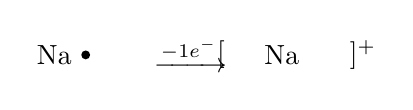
\begin{tikzpicture}[baseline=(Na.base),node distance=1.2cm]
% Neutral sodium atom (1 valence electron)
\node (Na) {\(\mathrm{Na}\)};

% One unpaired valence electron
\fill ($(Na.center)+(0.4,0)$) circle (1.6pt);

% Arrow and electron loss notation
\node[right=0.8cm of Na] (arrow) {\(\xrightarrow{- 1e^-}\)};

% Opening bracket for sodium ion
\node[right=1.6cm of Na] {\([\)};

% Sodium ion Na⁺ (0 valence electrons)
\node[right=2.2cm of Na] (Np) {\(\mathrm{Na}\)};

% Closing bracket and charge notation
\node[right=0.4cm of Np] {\(]^{+}\)};
\end{tikzpicture}

Answer: $\mathrm{Na^{+}}$ — electron removed, no valence dots, charge $+1$. \\
\hline
\end{tabular}

\newpage
\noindent
{\large\textbf{Content (fully worked out problems \& answers) continued...}}\\[0.2em]
\vspace{0.2cm}
\begin{tabular}{|p{0.9\linewidth}|}
\hline
\vspace{0.2cm}
\textbf{(77)} Given the Lewis dot for a neutral chlorine atom, draw the Lewis dot structure for the chloride ion, $\mathrm{Cl^-}$. Show where the added electron is and indicate the charge. \\
\hline
\vspace{0.2cm}
\textbf{Solution:} \\
Neutral Cl has 7 valence electrons (7 dots). Adding one electron gives 8 (octet) and a $-1$ charge. \\



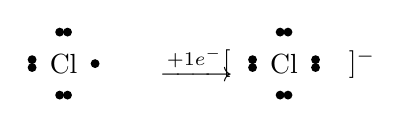
\begin{tikzpicture}[baseline=(Cln.base),node distance=1.25cm]
% Neutral chlorine atom (7 valence electrons: 3 lone pairs + 1 unpaired)
\node (Cln) {\(\mathrm{Cl}\)};

% Top lone pair (2 electrons side by side)
\fill ($(Cln.center)+(-0.05,0.4)$) circle (1.6pt);
\fill ($(Cln.center)+(0.05,0.4)$) circle (1.6pt);

% Left lone pair (2 electrons side by side)
\fill ($(Cln.center)+(-0.4,-0.05)$) circle (1.6pt);
\fill ($(Cln.center)+(-0.4,0.05)$) circle (1.6pt);

% Bottom lone pair (2 electrons side by side)
\fill ($(Cln.center)+(-0.05,-0.4)$) circle (1.6pt);
\fill ($(Cln.center)+(0.05,-0.4)$) circle (1.6pt);

% Right unpaired electron
\fill ($(Cln.center)+(0.4,0)$) circle (1.6pt);

% Arrow and electron addition notation
\node[right=0.8cm of Cln] (arrow) {\(\xrightarrow{+ 1e^-}\)};

% Opening bracket for chloride ion
\node[right=1.6cm of Cln] {\([\)};

% Chloride ion Cl⁻ (8 valence electrons: 4 lone pairs)
\node[right=2.2cm of Cln] (Cli) {\(\mathrm{Cl}\)};

% Top lone pair (side by side)
\fill ($(Cli.center)+(-0.05,0.4)$) circle (1.6pt);
\fill ($(Cli.center)+(0.05,0.4)$) circle (1.6pt);

% Right lone pair (side by side)
\fill ($(Cli.center)+(0.4,-0.05)$) circle (1.6pt);
\fill ($(Cli.center)+(0.4,0.05)$) circle (1.6pt);

% Bottom lone pair (side by side)
\fill ($(Cli.center)+(-0.05,-0.4)$) circle (1.6pt);
\fill ($(Cli.center)+(0.05,-0.4)$) circle (1.6pt);

% Left lone pair (side by side)
\fill ($(Cli.center)+(-0.4,-0.05)$) circle (1.6pt);
\fill ($(Cli.center)+(-0.4,0.05)$) circle (1.6pt);

% Closing bracket and charge notation
\node[right=0.4cm of Cli] {\(]^{-}\)};
\end{tikzpicture}

Answer: $\mathrm{Cl^-}$ — octet completed, charge $-1$. \\
\hline
\end{tabular}

\newpage
\noindent
{\large\textbf{Content (fully worked out problems \& answers) continued...}}\\[0.2em]
\vspace{0.2cm}

\begin{tabular}{|p{0.9\linewidth}|}
\hline
\vspace{0.2cm}
\textbf{(78)} Start from the Lewis dot of a neutral sulfur atom (S) and draw the Lewis dot structure for the sulfide ion, $\mathrm{S^{2-}}$. Show electron counting and charge. \\
\hline
\vspace{0.2cm}
\textbf{Solution:} \\
Neutral S has 6 valence electrons. Adding 2 electrons yields 8 (octet) and a $-2$ charge. \\


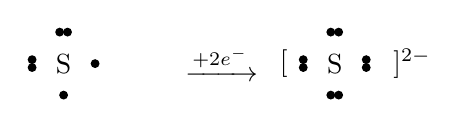
\begin{tikzpicture}[node distance=2cm]
% Neutral sulfur atom (6 valence electrons: 2 lone pairs + 2 unpaired)
\node (Sn) {\(\mathrm{S}\)};

% Top lone pair (2 electrons side by side)
\fill ($(Sn.center)+(-0.05,0.4)$) circle (1.6pt);
\fill ($(Sn.center)+(0.05,0.4)$) circle (1.6pt);

% Left lone pair (2 electrons side by side)
\fill ($(Sn.center)+(-0.4,-0.05)$) circle (1.6pt);
\fill ($(Sn.center)+(-0.4,0.05)$) circle (1.6pt);

% Right unpaired electron
\fill ($(Sn.center)+(0.4,0)$) circle (1.6pt);

% Bottom unpaired electron  
\fill ($(Sn.center)+(0,-0.4)$) circle (1.6pt);

% Arrow and addition notation
\node[right=1.2cm of Sn] (arrow) {\(\xrightarrow{+ 2e^-}\)};

% Opening bracket for sulfide ion
\node[right=2.4cm of Sn] {\([\)};

% Sulfide ion S²⁻ (8 valence electrons: 4 lone pairs)
\node[right=3cm of Sn] (Si) {\(\mathrm{S}\)};

% Top lone pair (side by side)
\fill ($(Si.center)+(-0.05,0.4)$) circle (1.6pt);
\fill ($(Si.center)+(0.05,0.4)$) circle (1.6pt);

% Right lone pair (side by side)
\fill ($(Si.center)+(0.4,-0.05)$) circle (1.6pt);
\fill ($(Si.center)+(0.4,0.05)$) circle (1.6pt);

% Bottom lone pair (side by side)
\fill ($(Si.center)+(-0.05,-0.4)$) circle (1.6pt);
\fill ($(Si.center)+(0.05,-0.4)$) circle (1.6pt);

% Left lone pair (side by side)
\fill ($(Si.center)+(-0.4,-0.05)$) circle (1.6pt);
\fill ($(Si.center)+(-0.4,0.05)$) circle (1.6pt);

% Closing bracket and charge notation
\node[right=0.4cm of Si] {\(]^{2-}\)};
\end{tikzpicture}




Answer: $\mathrm{S^{2-}}$ — octet, charge $-2$. \\
\hline
\end{tabular}

\newpage
\noindent
{\large\textbf{Content (fully worked out problems \& answers) continued...}}\\[0.2em]
\vspace{0.2cm}

\begin{tabular}{|p{0.9\linewidth}|}
\hline
\vspace{0.2cm}
\textbf{(79)} Given the Lewis dot of a neutral magnesium atom (Mg), draw the Lewis structure for $\mathrm{Mg^{2+}}$. Indicate removal of valence electrons and the resulting charge. \\
\hline
\vspace{0.2cm}
\textbf{Solution:} \\
Neutral Mg has 2 valence electrons (two dots). Removing both gives Mg$^{2+}$ with no valence dots and a $+2$ charge. \\




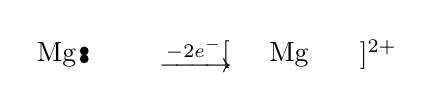
\begin{tikzpicture}[baseline=(Mg.base),node distance=1.2cm]
% Neutral magnesium atom (2 valence electrons)
\node (Mg) {\(\mathrm{Mg}\)};

% One lone pair (2 electrons side by side)
\fill ($(Mg.center)+(0.35,0.05)$) circle (1.6pt);
\fill ($(Mg.center)+(0.35,-0.05)$) circle (1.6pt);

% Arrow and electron loss notation
\node[right=0.8cm of Mg] (arrow) {\(\xrightarrow{- 2e^-}\)};

% Opening bracket for magnesium ion
\node[right=1.6cm of Mg] {\([\)};

% Magnesium ion Mg²⁺ (0 valence electrons)
\node[right=2.2cm of Mg] (Mgi) {\(\mathrm{Mg}\)};

% Closing bracket and charge notation
\node[right=0.4cm of Mgi] {\(]^{2+}\)};
\end{tikzpicture}


Answer: $\mathrm{Mg^{2+}}$ — two electrons removed, charge $+2$. \\
\hline
\end{tabular}

\newpage
\noindent
{\large\textbf{Content (fully worked out problems \& answers) continued...}}\\[0.2em]
\vspace{0.2cm}

\begin{tabular}{|p{0.9\linewidth}|}
\hline
\vspace{0.2cm}
\textbf{(80)} Start from the Lewis dot for a neutral copper atom (showing its single 4s valence electron as one dot) and draw the Lewis structure for the cuprous ion, $\mathrm{Cu^{+}}$. Explain briefly. \\
\hline
\vspace{0.2cm}
\textbf{Solution:} \\
A common simple Lewis-dot convention places one valence dot for Cu (4s$^1$). Removing that electron gives Cu$^+$ with no valence dot and charge $+1$. (Note: d-electrons are not shown in simple Lewis-dot for many transition metals.) \\




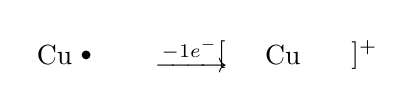
\begin{tikzpicture}[baseline=(Cu.base),node distance=1.2cm]
% Neutral copper atom (1 valence electron)
\node (Cu) {\(\mathrm{Cu}\)};

% One unpaired valence electron
\fill ($(Cu.center)+(0.4,0)$) circle (1.6pt);

% Arrow and electron loss notation
\node[right=0.8cm of Cu] (arrow) {\(\xrightarrow{- 1e^-}\)};

% Opening bracket for copper ion
\node[right=1.6cm of Cu] {\([\)};

% Copper ion Cu⁺ (0 valence electrons)
\node[right=2.2cm of Cu] (Cui) {\(\mathrm{Cu}\)};

% Closing bracket and charge notation
\node[right=0.4cm of Cui] {\(]^{+}\)};
\end{tikzpicture}


Answer: $\mathrm{Cu^{+}}$ — 4s electron removed, no valence dot, charge $+1$. \\
\hline
\end{tabular}

\newpage
\noindent
{\large\textbf{Content (fully worked out problems \& answers) continued...}}\\[0.2em]
\vspace{0.2cm}

\begin{tabular}{|p{0.9\linewidth}|}
\hline
\vspace{0.2cm}
\textbf{(81)} Given the Lewis dot for neutral nitrogen (N), draw the Lewis dot for nitride ion, $\mathrm{N^{3-}}$, and indicate electron counting and charge. \\
\hline
\vspace{0.2cm}
\textbf{Solution:} \\
Neutral N has 5 valence electrons (5 dots). Adding 3 electrons yields 8 (octet) and a $-3$ charge. \\



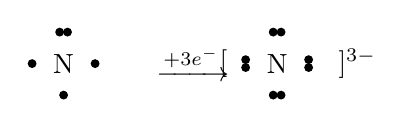
\begin{tikzpicture}[baseline=(N.base),node distance=1.15cm]
% Neutral nitrogen atom (5 valence electrons: 1 lone pair + 3 unpaired)
\node (N) {\(\mathrm{N}\)};

% Top lone pair (2 electrons side by side)
\fill ($(N.center)+(-0.05,0.4)$) circle (1.6pt);
\fill ($(N.center)+(0.05,0.4)$) circle (1.6pt);

% Right unpaired electron
\fill ($(N.center)+(0.4,0)$) circle (1.6pt);

% Bottom unpaired electron  
\fill ($(N.center)+(0,-0.4)$) circle (1.6pt);

% Left unpaired electron
\fill ($(N.center)+(-0.4,0)$) circle (1.6pt);

% Arrow and addition notation
\node[right=0.8cm of N] (arrow) {\(\xrightarrow{+ 3e^-}\)};

% Opening bracket for nitride ion
\node[right=1.6cm of N] {\([\)};

% Nitride ion N³⁻ (8 valence electrons: 4 lone pairs)
\node[right=2.2cm of N] (Ni) {\(\mathrm{N}\)};

% Top lone pair (side by side)
\fill ($(Ni.center)+(-0.05,0.4)$) circle (1.6pt);
\fill ($(Ni.center)+(0.05,0.4)$) circle (1.6pt);

% Right lone pair (side by side)
\fill ($(Ni.center)+(0.4,-0.05)$) circle (1.6pt);
\fill ($(Ni.center)+(0.4,0.05)$) circle (1.6pt);

% Bottom lone pair (side by side)
\fill ($(Ni.center)+(-0.05,-0.4)$) circle (1.6pt);
\fill ($(Ni.center)+(0.05,-0.4)$) circle (1.6pt);

% Left lone pair (side by side)
\fill ($(Ni.center)+(-0.4,-0.05)$) circle (1.6pt);
\fill ($(Ni.center)+(-0.4,0.05)$) circle (1.6pt);

% Closing bracket and charge notation
\node[right=0.4cm of Ni] {\(]^{3-}\)};
\end{tikzpicture}


Answer: $\mathrm{N^{3-}}$ — octet filled, charge $-3$. \\
\hline
\end{tabular}
\newpage
\section*{\underline{Activity 1}}
\vspace{0.2cm}
\begin{tabular}{|p{4.2cm}|p{9.8cm}|}
\hline
\textbf{Collaborative Learning Techniques} & Group Discussion\\
\hline
\textbf{Learning Strategy} & Vocabulary Development \\
\hline
\textbf{Time} & 12:10---12:30\\
\hline
\textbf{Materials} & Notes \\
\hline
\textbf{Lecture/Textbook/Old Plans/Slide References} & Chapter 3: Periodic Table\\
\hline
\end{tabular}

\vspace{0.5cm}

{\large\textbf{Definition}}\\
\noindent
\begin{tabular}{|p{0.9\linewidth}|}
\hline
\begin{enumerate}
    \item\textbf{Group Discussion:} One person in the group is asked to present on a topic or review material for the group and then lead the discussion for the group. This person should not be the regular group leader.
    \item\textbf{Vocabulary Development:} Chunking related terms into meaningful groups can be more helpful than drilling students on exact definitions. Compose a list of key terms from the lecture rangin in levels of specificity, Scramble the terms and then encourage pairs of students to organize the terms into serveral categories that are meaninful to them. Then have them define or give an example of terms where appropriate. Finally, have each pair discuss their categories with the entire group. Get the students to check spelling.
 
\end{enumerate}\\
\hline
\end{tabular}
\vspace{0.2cm}
\newpage
{\large\textbf{Instructions (please provide a\hl{DETAILED} activity breakdown below (and/or attached}}\\
\noindent
\begin{tabular}{|p{0.9\linewidth}|}
\hline
\vspace{0.2cm}
\begin{enumerate}
    \item \textbf{Form a Circle:} All students sit or stand in a circle so that everyone can see and interact with each other.
    \item \textbf{Prepare Terms by Specificity:} Compose a comprehensive list of key terms related to ions, atomic orbitals, molecules, bonds, elements, isotopes, measurements, electron configuration, and VSEPR. Organize terms into levels of specificity:
    \begin{itemize}
        \item \textit{Level 1 – Broad Concepts:} e.g., “element,” “molecule”
        \item \textit{Level 2 – Intermediate Concepts:} e.g., “cation,” “polar covalent bond,” “2p orbital”
        \item \textit{Level 3 – Specific Examples:} e.g., “Na+,” “H–Cl bond,” “sp$^2$ hybridization”
    \end{itemize}
    \item \textbf{Scramble and Distribute:} Shuffle the terms and give each student or pair a subset to organize within the specificity levels.
    \item \textbf{Round-Robin Discussion:} Moving around the circle, each student or pair presents their terms starting from the broadest level to the most specific. For each term, they provide a definition or example.  
    \item \textbf{Peer Verification:} Other students in the circle can suggest corrections, alternative examples, or clarifications. Emphasize discussion rather than right/wrong answers.
    \item \textbf{Spelling and Accuracy Check:} Ensure terms are spelled correctly and scientifically accurate. The instructor or SI leader monitors and provides guidance.
    \item \textbf{Reflection:} After all terms are discussed, students reflect on the hierarchical relationships between concepts, noting how broad categories encompass intermediate and specific examples.
\end{enumerate} \\
\hline
\end{tabular}

\newpage
{\large\textbf{Checking for Understanding (general conceptual questions)}}\\
\noindent \begin{tabular}{|p{0.9\linewidth}|}
\hline
\vspace{0.2cm}
\begin{enumerate}
    \item How do you identify cations and anions, and what processes form them?
    \item How can electron configurations predict the chemical behavior and reactivity of elements?
    \item What is the difference between an atom, an ion, and an isotope, and how do these differences affect chemical properties?
    \item How do orbitals differ from orbits, and why is this distinction important for understanding electron arrangements?
    \item How can you determine the shape of a molecule using VSEPR theory?
    \item What is the difference between ionic, polar covalent, and nonpolar covalent bonds, and how can you predict which will form?
    \item How do electronegativity differences relate to bond polarity and molecular polarity?
    \item How do you determine if a molecule is polar or nonpolar overall?
    \item How do the number of protons, neutrons, and electrons determine the identity and charge of an atom or ion?
    \item How can you organize elements using the periodic table, and what patterns help predict properties?
    \item How does atomic and molecular structure influence physical properties such as density or polarity?
    \item How do measurements in chemistry, such as mass, volume, and concentration, relate to chemical calculations and formulas?
    \item How do isotopes of the same element differ in mass but retain the same chemical behavior?
    \item How do specific orbitals (s, p, d, f) relate to electron distribution in atoms and the periodic trends?
    \item How do scientific notation and powers of ten help when representing very large or very small quantities in chemistry?
\end{enumerate}
\\
\hline
\end{tabular}
\newpage

\noindent
\section*{\underline{Activity 2}}
\begin{tabular}{|p{4.5cm}|p{9.5cm}|}
\hline
\textbf{Collaborative Learning Techniques} & Jigsaw \\
\hline
\textbf{Learning Strategy} &  Boardwork Model (modified)\\
\hline
\textbf{Time} & 12:30---12:50\\
\hline
\textbf{Materials} & Colored whiteboard markers, a whiteboard, partitioned questions (to display multiple to multiple groups at a time).\\
\hline
\textbf{Lecture/Textbook/Old Plans/Slide References} & Chapter 1: Basics of Matter, Chapter 2: Measurements\\
\hline
\end{tabular}

\vspace{0.5cm}
\noindent
\begin{tabular}{|p{0.9\linewidth}|}
\hline
{\large\textbf{Definitions}}
\begin{enumerate}
   \item\textbf{Jigsaw:} Jigsaws, when used properly, make the group as a whole dependent upon all of them in subgroups. Each group provides a peice of the puzzle. Group members are broken into smaller groups. Each small group works on some aspect of the same problem, question, or issue. They then share their part of the puzzle with the large group.
   \item\textbf{Boardwork Model:} This is a method of organizing boardwork in order to fascilitate an undertsanding of problem-solving strategies. The baord should be divdied into 4 sections: 1.) Prerequisite Knowledge, 2.) Mathematical Steps, 3.) Narrative of the Steps, 4.) Additional Sample Problem. Encourage one student to fill out section 1 on the board. Then encourage 2 students to simultaneously complete section 2 and 3 on the board. Lastly, have another student complete section 4. Encourage the students to use this model when studying outside of the SI session.
\end{enumerate}
\\ \hline
\end{tabular}
\newpage
{\large\textbf{Instructions (please provide a\hl{DETAILED} activity breakdown below (and/or attached)}}\\
\noindent
\begin{tabular}{|p{0.9\linewidth}|}
\hline
\vspace{0.2cm}
\textbf{Objective:} Guide students to work independently on a chemistry worksheet, solving problems. After asking a survey for answers completing each piece, students share their solutions and recieve feedback on each step to ensure understanding before proceeding.  
\vspace{0.2cm}

\textbf{Setup:}  
\begin{itemize}  
    \item Prepare a worksheet divided into sections or “pieces,” each containing a set of chemistry problems (e.g., ions, electron configuration, molecular geometry, bonding, measurements).  
    \item Each piece should build upon the previous one to create a logical progression from broad to specific concepts.  
    \item Provide reference materials (periodic table, formulas, or charts) as needed.  
    \item Ensure students have paper, pencils, and optionally colored pens for diagrams or drawings.  
\end{itemize}  

\textbf{Running the Activity:}  
\begin{enumerate}  
    \item Explain that students will complete the worksheet **piece by piece**, solving each section on their own first.  
    \item After finishing a piece, students **share their answers** with a partner or small group to check understanding.  
    \item Students discuss each solution, correcting errors or clarifying concepts before moving to the next piece.  
    \item Once all students confirm understanding of the current piece, they move to the next section of the worksheet.  
    \item Continue this process until the entire worksheet is completed.  
    \item Encourage students to annotate their worksheets with notes from peer discussions to reinforce learning.  
\end{enumerate}  

\textbf{Facilitator Role:}  
\begin{itemize}  
    \item Circulate to monitor student progress and understanding.  
    \item Provide hints or clarification without giving away solutions.  
    \item Ensure students are actively discussing and verifying each piece before moving on.  
    \item Take note of common misunderstandings for future review or debriefing.  
    \item At the end, lead a brief class discussion summarizing key concepts and connections between the worksheet sections.  
\end{itemize}  
\vspace{0.2cm}
\\ \hline
\end{tabular}
\newpage

\newpage
\noindent
{\large\textbf{Checking for Understanding (questions \& answers)}}\\[0.2em]
\noindent
\begin{tabular}{|p{0.9\linewidth}|}
\hline
\textbf{Questions:} \\
\begin{enumerate}
    \item How does solving the worksheet in sequential “pieces” help students build understanding step by step?  
    \item Why is sharing answers with peers after each piece beneficial for learning chemistry concepts?  
    \item In what ways does this approach encourage students to actively reflect on their own understanding?  
    \item How can verifying each piece with a partner prevent misconceptions from carrying forward?  
    \item How does this method promote independent problem-solving skills while still incorporating collaboration?  
    \item What strategies can students use to interpret and categorize chemistry terms as they work through the worksheet?  
    \item How does this sequential, piece-by-piece approach help students make connections between broad and specific concepts (e.g., elements → ions → orbitals → molecules)?  
    \item How can discussing each piece improve students’ ability to explain chemical reasoning clearly?  
    \item What advantages do students gain from seeing multiple approaches to the same problem or term?  
    \item How does this model help students practice applying theoretical knowledge to concrete problems?  
    \item In what ways can the instructor or SI leader use this approach to identify areas where students struggle?  
    \item How does completing the worksheet in pieces enhance retention of chemistry concepts for students with varying levels of prior knowledge?  
\end{enumerate} \\
\hline  
\end{tabular}

\newpage
\noindent
\section*{\underline{Closer}}
\begin{tabular}{|p{4.2cm}|p{9.8cm}|}
\hline
\textbf{Collaborative Learning Techniques} & Group Survey\\
\hline
\textbf{Learning Strategy} & Brain dump\\
\hline
\textbf{Time} & 12:50---12:55\\
\hline
\textbf{Materials} & Index cards, writing utensils\\
\hline
\textbf{Lecture/Textbook/Old Plans/Slide References} & Chapter 1: Basics of Matter, Chapter 2: Measurements\\
\hline
\end{tabular}

\vspace{0.5cm}
\noindent
\begin{tabular}{|p{0.9\linewidth}|}
\hline
{\large\textbf{Definitions}}
\begin{enumerate}
   \item\textbf{Group survey:} Each group member is surveyed to discover their position on an issue, problem or topic. This process ensures that each member of the group is allowed to offer or state their point of view.
   \item\textbf{Brain dump:} This is a great closer for students to sum up their knowledge on the topic(s) from the session. Have the students take out a blank piece of paper /Google Doc and write/type("dump") everything they know relevant from the discussion that day. The SI Leader can look at their work to assess the students' understanding of the course material and have them compare it to each other. It is important to at least discuss with the students so the SI Leader knows the students' comfort levels with the material. 
\end{enumerate}
\\ \hline
\end{tabular}

\newpage
\noindent
{\large\textbf{Instructions (please provide a\hl{DETAILED} activity breakdown below (and/or attached}}

\begin{tabular}{|p{0.9\linewidth}|}
\hline
\begin{enumerate}[itemsep=0.3em]
   \item Students are put into small groups and are asked to write down their confidence on a single notecard without names.
   \item The cards are evidence of the group's confidence in the content.
\end{enumerate}
\\ \hline
\end{tabular}

\vspace{0.5cm}
\noindent
{\large\textbf{Content (fully worked out problems \& answers)}

\begin{tabular}{|p{0.9\linewidth}|}
\hline
\begin{itemize}
   \item No new worked problems; brain dump.
\end{itemize}
\\ \hline
\end{tabular}

\vspace{0.5cm}
\noindent
{\large\textbf{Checking for Understanding (questions \& answers) continued...}

\begin{tabular}{|p{0.9\linewidth}|}
\hline
\begin{itemize}
   \item Review confidence levels
   \item Interpret the variety of confidence and their distribution in groups.
\end{itemize}
\\ \hline
\end{tabular}
\newpage
\section*{Plan Checklist}

\begin{tabular}{|p{0.9\linewidth}|}
\hline
\begin{itemize}
\item[$\Box$] Variety of Collaborative Learning Techniques and Learning Strategies
\item[$\Box$] Chapter/slide\# where information is coming from
\item[$\Box$] Included timestamps (and buffer time as needed)
\item[$\Box$] Details on how leader will break up students
\item[$\Box$] Checking for Understanding questions
\item[$\Box$] Fully worked out problems and examples for each activity
\item[$\Box$] Necessary links required for online implementation (if applicable)
\item[$\Box$] Source material correctly cited (if applicable)
\item[$\Box$] Plan is uploaded to Teams
\end{itemize}
\\ \hline
\end{tabular}
\newpage

\end{document}
